%\documentclass[a4,semhelv,landscape]{seminar}
\documentclass[landscape]{slides}
%\documentclass[pdf, default, slideBW, nocolorBG]{prosper}
\usepackage[left=0.2cm,top=0.2cm,right=0.2cm,bottom=0.2cm,nohead,nofoot]{geometry}
%\def\everyslide{\sffamily}
%\usepackage{fullpage}
\usepackage{graphicx}
\usepackage[usenames]{color}
%\usepackage{color}
\usepackage{verbatim}
\usepackage{nopageno}
\usepackage{setspace}
%\usepackage{times}
% define some nice colors
\definecolor{myred}{rgb}{0.6,0,0}
\definecolor{myblue}{rgb}{0,0.2,0.4}
\definecolor{mygreen}{rgb}{0,0.5,0.0}
\definecolor{mypurple}{cmyk}{0.5,1.0,0.0,0.0}
%\color{myblue}

\begin{document}
%%%%%%%%%%%%%%%%%%%%%%%%%%%%%%%%%%%%%%%%%%%%%%%%%%%%%%%%%%%%%%%%%%%%
%Slide 0 - title
\begin{slide}
\begin{center}
\large{\textbf{Modeling structural RNA families with Infernal}}

\normalsize

Eric Nawrocki \\

\medskip

\medskip

\medskip

\medskip

\medskip

\small
\begin{tabular}{c}
Alejandro Sch\"{a}ffer's group \\
\\
National Center for Biotechnology Information\\
National Institutes of Health\\
\\
Howard Hughes Medical Institute \\ 
Janelia Research Campus \\
\end{tabular}

\vspace{0.1in}


\includegraphics[width=2.5in]{figs/ncbi-logo}
\hspace{1in}
\includegraphics[width=2.5in]{figs/jrc-color}

\end{center}
\end{slide}
%%%%%%%%%%%%%%%%%%%%%%%%%%%%%%%%%%%%%%%%%%%%%%%%%%%%%%%%%%%%%%%%%%%%%%
\begin{slide}
\begin{center}
{\bf Many functional RNAs adopt a conserved 3-dimensional 
  structure}

\medskip

Three representations of a transfer RNA:

%\includegraphics[width=10.5in]{figs/trna-123}
\includegraphics[width=9in]{figs/trna-123}

\end{center}

\vfill

\end{slide}
%%%%%%%%%%%%%%%%%%%%%%%%%%%%%%%%%%%%%%%%%%%%%%%%%%%%%%%%%%%%%%
\begin{slide}
\begin{center}
{\bf Many functional RNAs adopt a conserved 3-dimensional 
  structure}
\medskip

Three representations of a transfer RNA:

%\includegraphics[width=10.5in]{figs/trna-123}
\includegraphics[width=9in]{figs/trna-123}
\end{center}

\begin{itemize}
\item
  BLAST: given a single sequence, search genomes for similar sequences.
\item
  BLAST cannot take advantage of:
\begin{itemize}
  \item sequence conservation, which varies across the gene
  \item secondary structure
\end{itemize}
\end{itemize}

\vfill

\end{slide}
%%%%%%%%%%%%%%%%%%%%%%%%%%%%%%%%%%%%%%%%%%%%%%%%%%%%%%%%%%%%%
\begin{slide}
\begin{center}
%\textbf{Comparative analysis of sequence families}: \\
\textbf{Sequence conservation provides \\ information for homology searches}

\medskip
Conservation levels vary across alignment columns.

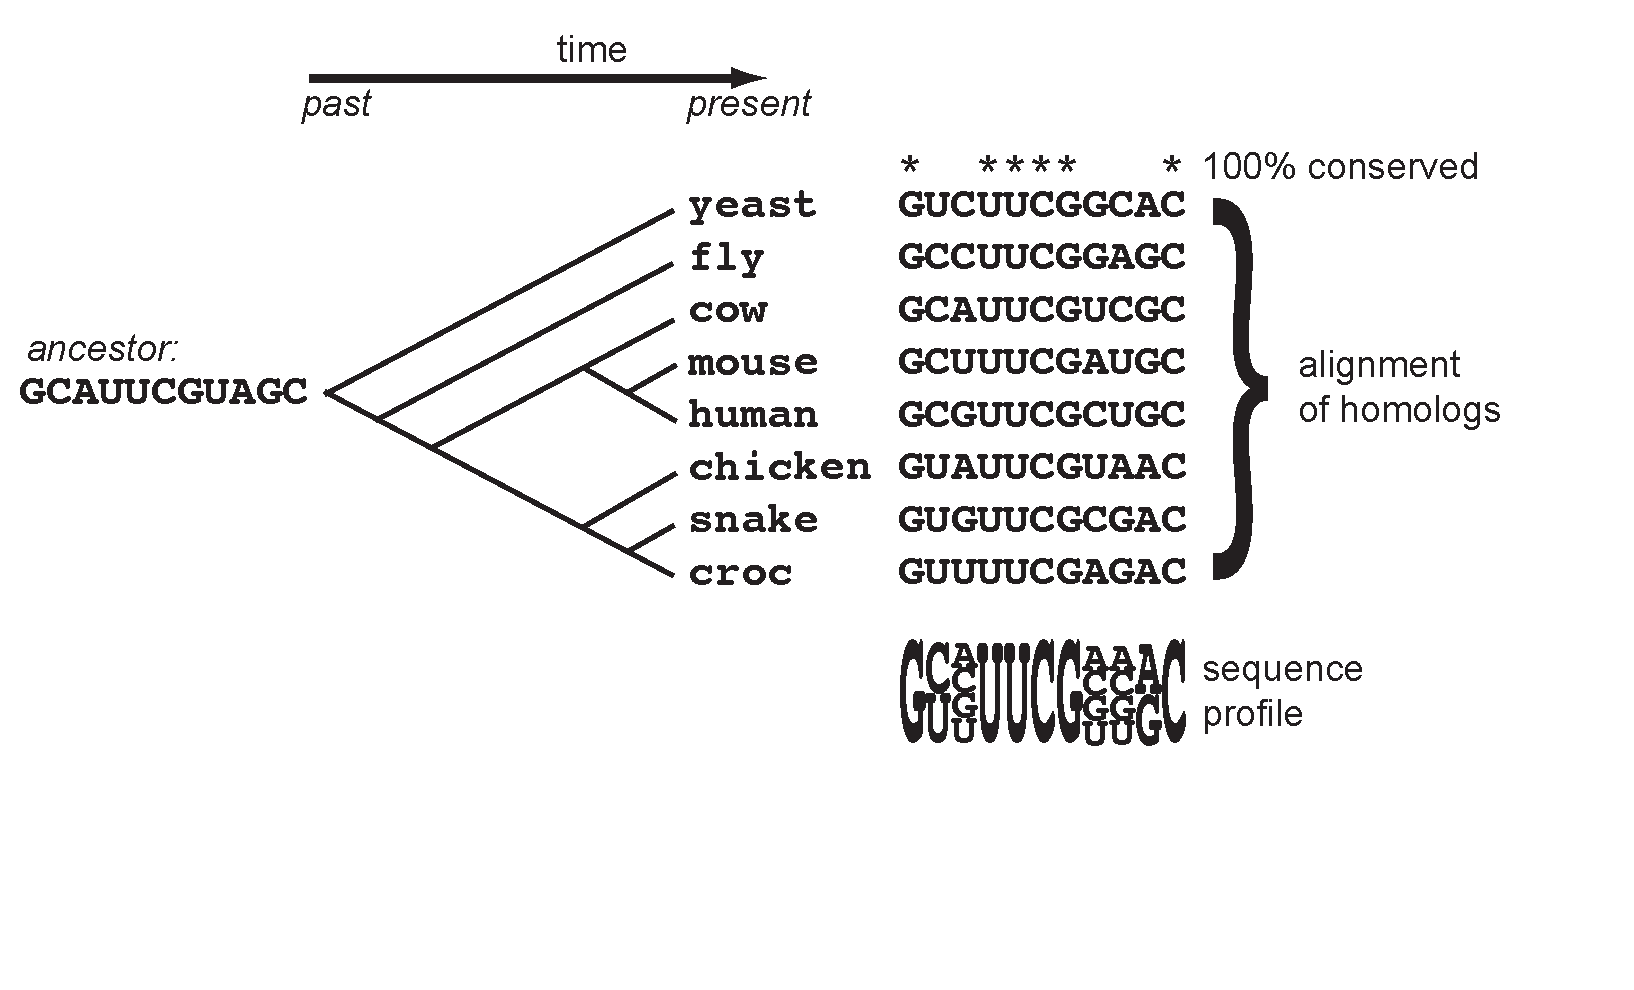
\includegraphics[width=10in]{figs/seqstructprofiles-seq1}
\end{center}

\vfill
\end{slide}
%%%%%%%%%%%%%%%%%%%%%%%%%%%%%%%%%%%%%%%%%%%%%%%%%%%%%%%%%%%%%%%%%%%%%%
\begin{slide}
\begin{center}
\textbf{Structure conservation provides additional information}
\medskip

Base-paired positions covary \\ to maintain Watson-Crick complementarity.

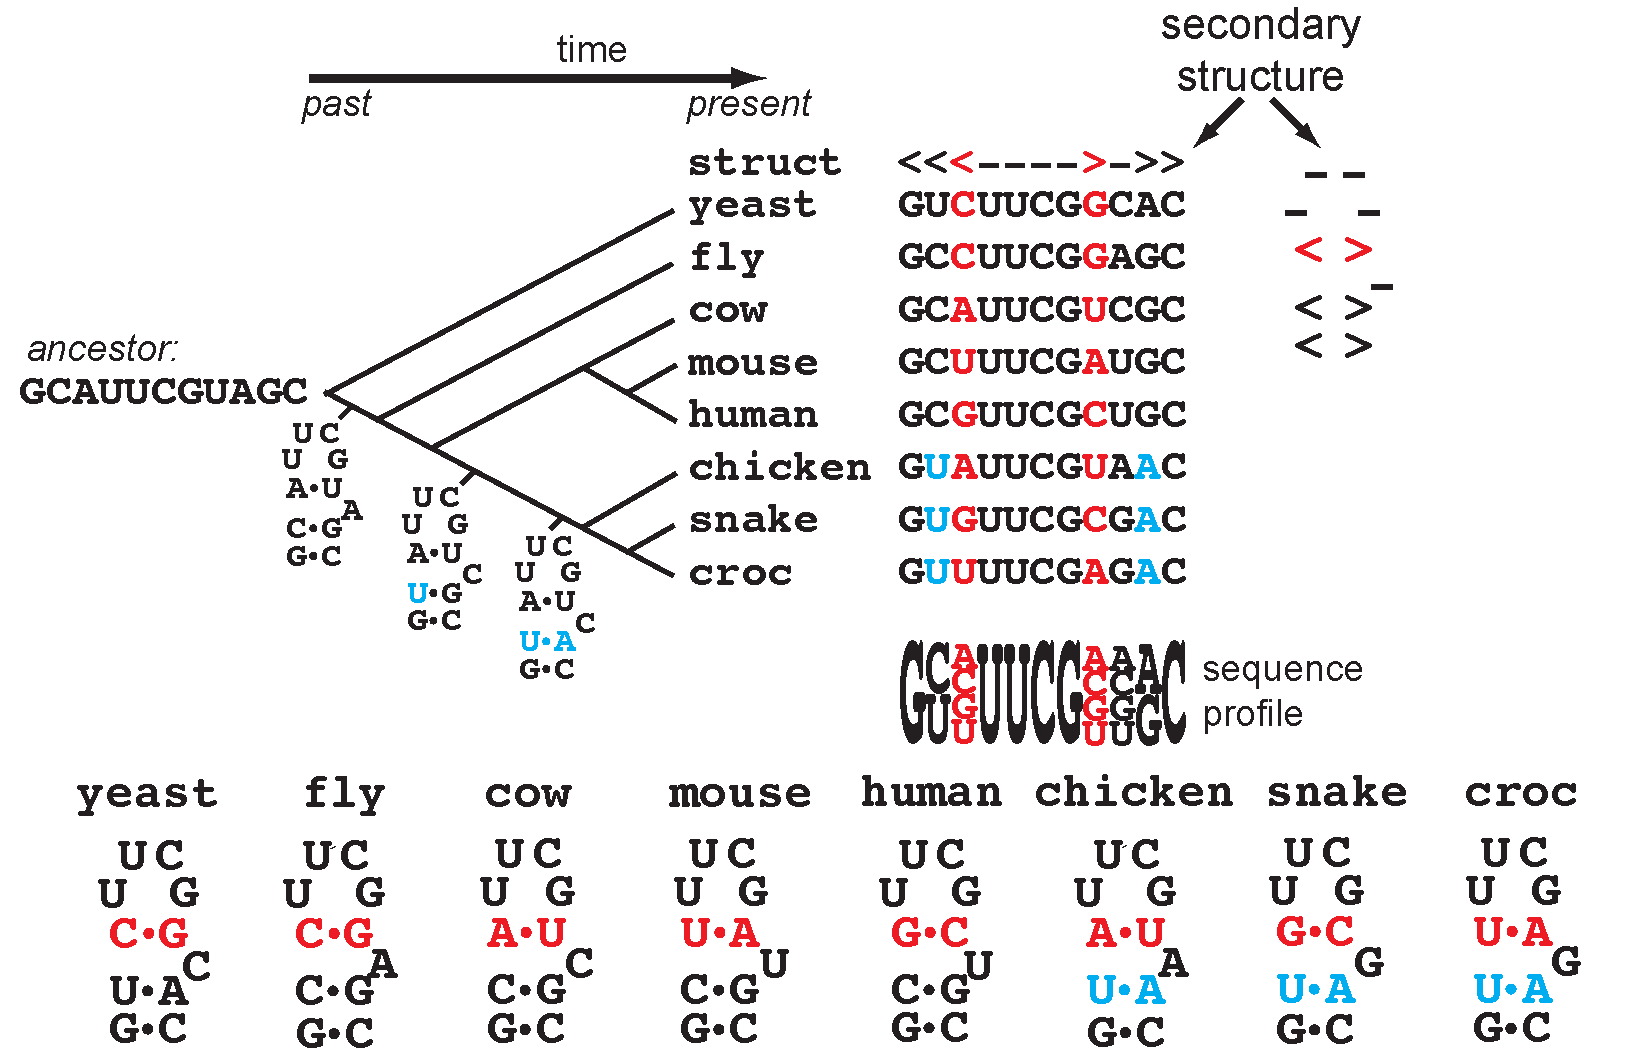
\includegraphics[width=10in]{figs/seqstructprofiles-struct2}
\end{center}

\vfill
\end{slide}
%%%%%%%%%%%%%%%%%%%%%%%%%%%%%%%%%%%%%%%%%%%%%%%%%%%%%%%%%%%%%%%%%%%%%%%%%%
\begin{slide}
\begin{center}
\textbf{Amount of information in a profile can be measured in bits}
\medskip

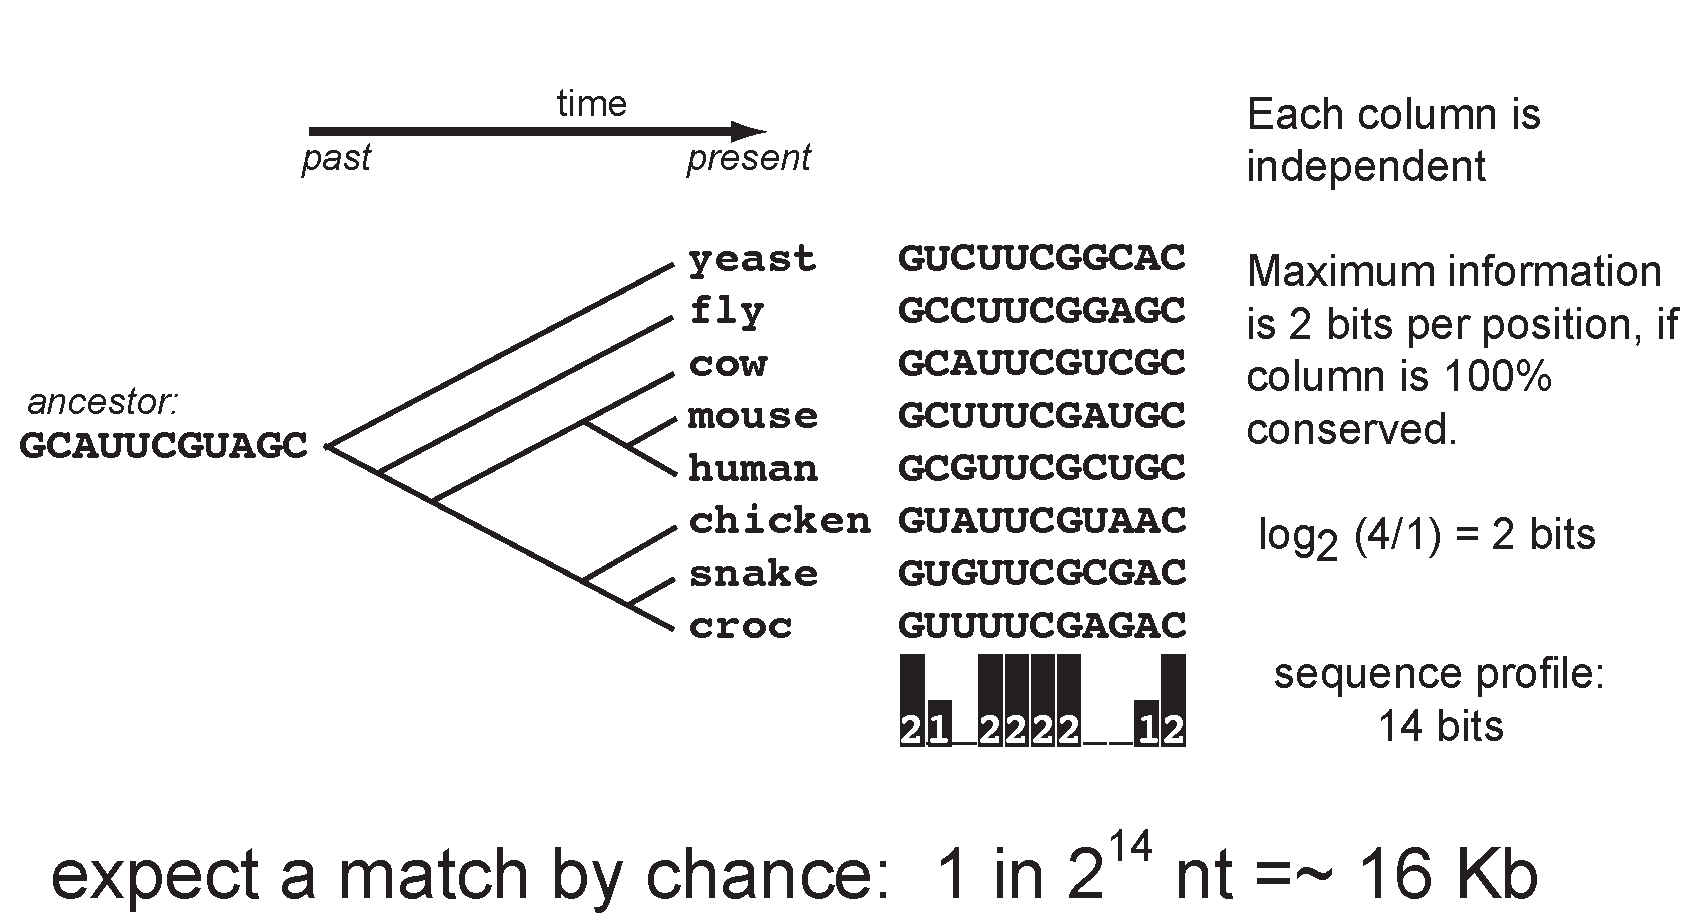
\includegraphics[width=9in]{figs/seqstructprofiles-2014-seqinfo}
\end{center}

\vfill
\end{slide}
%%%%%%%%%%%%%%%%%%%%%%%%%%%%%%%%%%%%%%%%%%%%%%%%%%%%%%%%%%%%%%%%%%%%%%%%%%
\begin{slide}
\begin{center}
\textbf{Structure contributes additional information from covariation}
\medskip

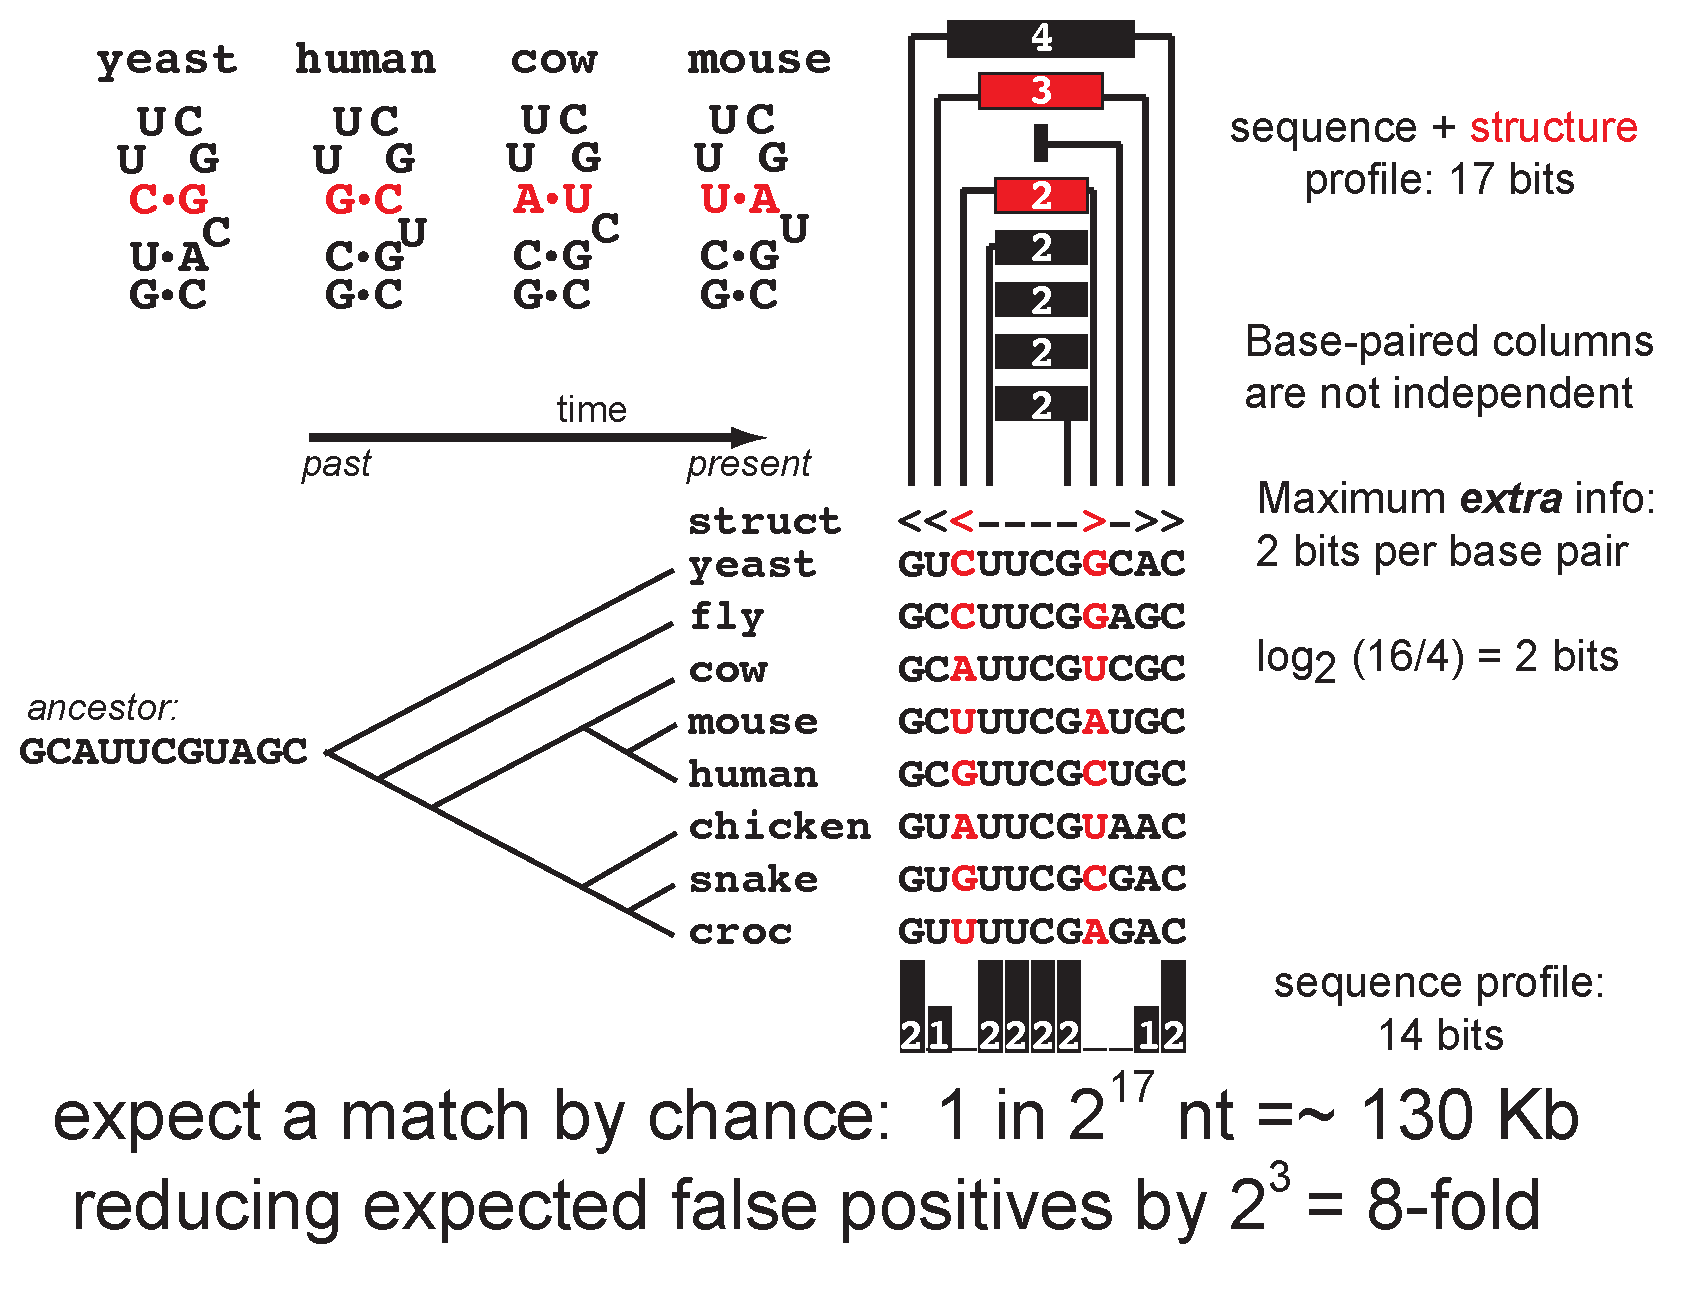
\includegraphics[width=9in]{figs/seqstructprofiles-2014-structinfo}
\end{center}

\vfill
\end{slide}
%%%%%%%%%%%%%%%%%%%%%%%%%%%%%%%%%%%%%%%%%%%%%%%%%%%%%%%%%%%%%%%%%%%%%%%%%%
\begin{slide}
\begin{center}
\textbf{Levels of sequence and structure conservation in RNA families}
\end{center}
\medskip

\begin{center}
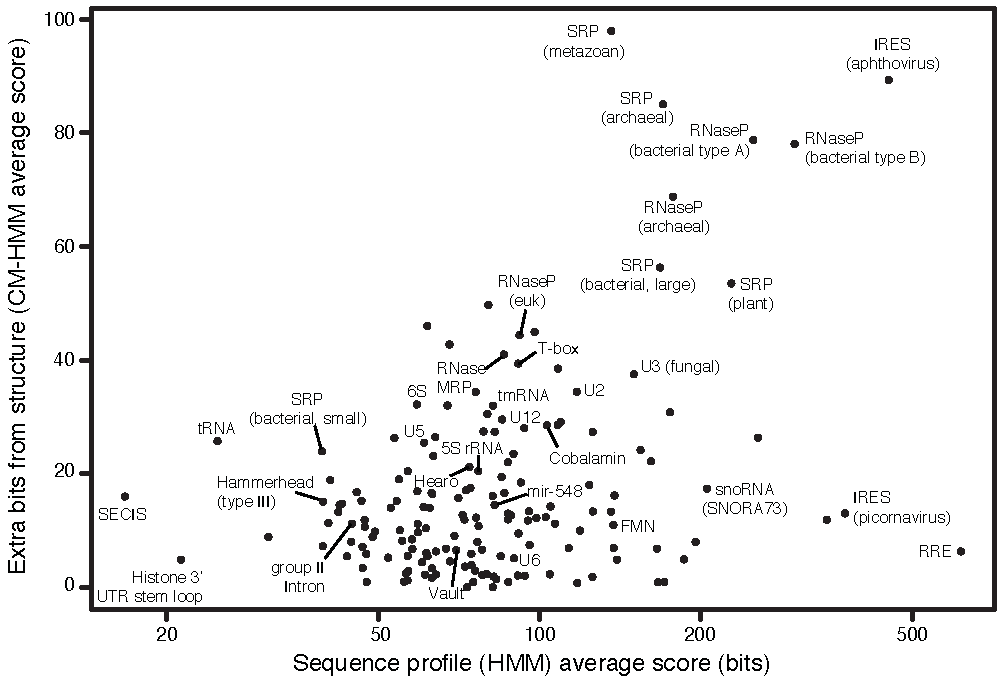
\includegraphics[height=6.5in]{figs/avgscores-rfam11}
\end{center}

\vfill

\end{slide}
%%%%%%%%%%%%%%%%%%%%%%%%%%%%%%%%%%%%%%%%%%%%%%%%%%%%%%%%%%%%%%%%%%%
\begin{slide}
\begin{center}
%\textbf{profile HMMs and covariance models}
\textbf{Eddy lab software for profile probabilistic models } (since 1994)
\end{center}
\medskip

\begin{center}
\small
\begin{tabular}{r|cc} 
%             &         & sequence \\
%             & sequence& and structure \\
%             & profiles& profiles \\ \hline
             & sequence & sequence and \\
             & profiles & structure profiles \\ \hline
  \\
  models     & profile HMMs     & {\color{red} covariance models (CMs)} \\ 
  \\
  software   & {\sc HMMER}      & {\sc Infernal} \\ 
  \\
  main use   & proteins,         & structural RNAs \\ 
             & repetitive DNA elements &  \\
  \\
  databases  & {\sc Pfam} and \sc{Dfam}       & {\sc Rfam} \\
             & (14831 and 1132 entries) & (2450 families) \\
  \\
%  primary sequence & yes & yes \\
%  \\
%  secondary structure & no & yes \\
%  \\
%  algorithms & Viterbi, Forward & CYK, Inside \\
%%             & Forward & Inside \\
%             &         & \\
%  complexity & $O(LN)$ & $O(LN^{2} log N)$ \\
%  \\
  performance& faster but    & slower but    \\
  for RNAs   & less accurate & more accurate \\
\end{tabular}

%\hspace{1.2in}\includegraphics[height=2in]{figs/hmmer_logo}\hspace{1.05in}\includegraphics[height=2.6in]{figs/infernal_logo}
\hspace{1.8in}
\includegraphics[height=2.7in]{figs/hmmer-infernal-refs-2015}

\end{center}

\vfill

\end{slide}
%%%%%%%%%%%%%%%%%%%%%%%%%%%%%%%%%%%%%%%%%%%%%%%%%%%%%%%%%%%%%%%
%%%%%%%%%%%%%%%%%%%%%%%%%%%%%%%%%%%%%%%%%%%%%%%%%%%%%%%%%%%%%%%
%%%%%%%%%%%%%%%%%%%%%%%%%%%%%%%%%%%%%%%%%%%%%%%%%%%%%%%%%%%%%%%
%%%%%%%%%%%%%%%%%%%%%%%%%%%%%%%%%%%%%%%%%%%%%%%%%%%%%%%%%%%%%%%
%%%%%%%%%%%%%%%%%%%%%%%%%%%%%%%%%%%%%%%%%%%%%%%%%%%%%%%%%%%%%%%
%%%%%%%%%%%%%%%%%%%%%%%%%%%%%%%%%%%%%%%%%%%%%%%%%%%%%%%%%%%%%%%
%%%%%%%%%%%%%%%%%%%%%%%%%%%%%%%%%%%%%%%%%%%%%%%%%%%%%%%%%%%%%%%%%%%%
\begin{slide}
\begin{center}
%\textbf{profile HMMs and covariance models}
\textbf{Profile HMMs: sequence family models built from alignments}
\end{center}

\center{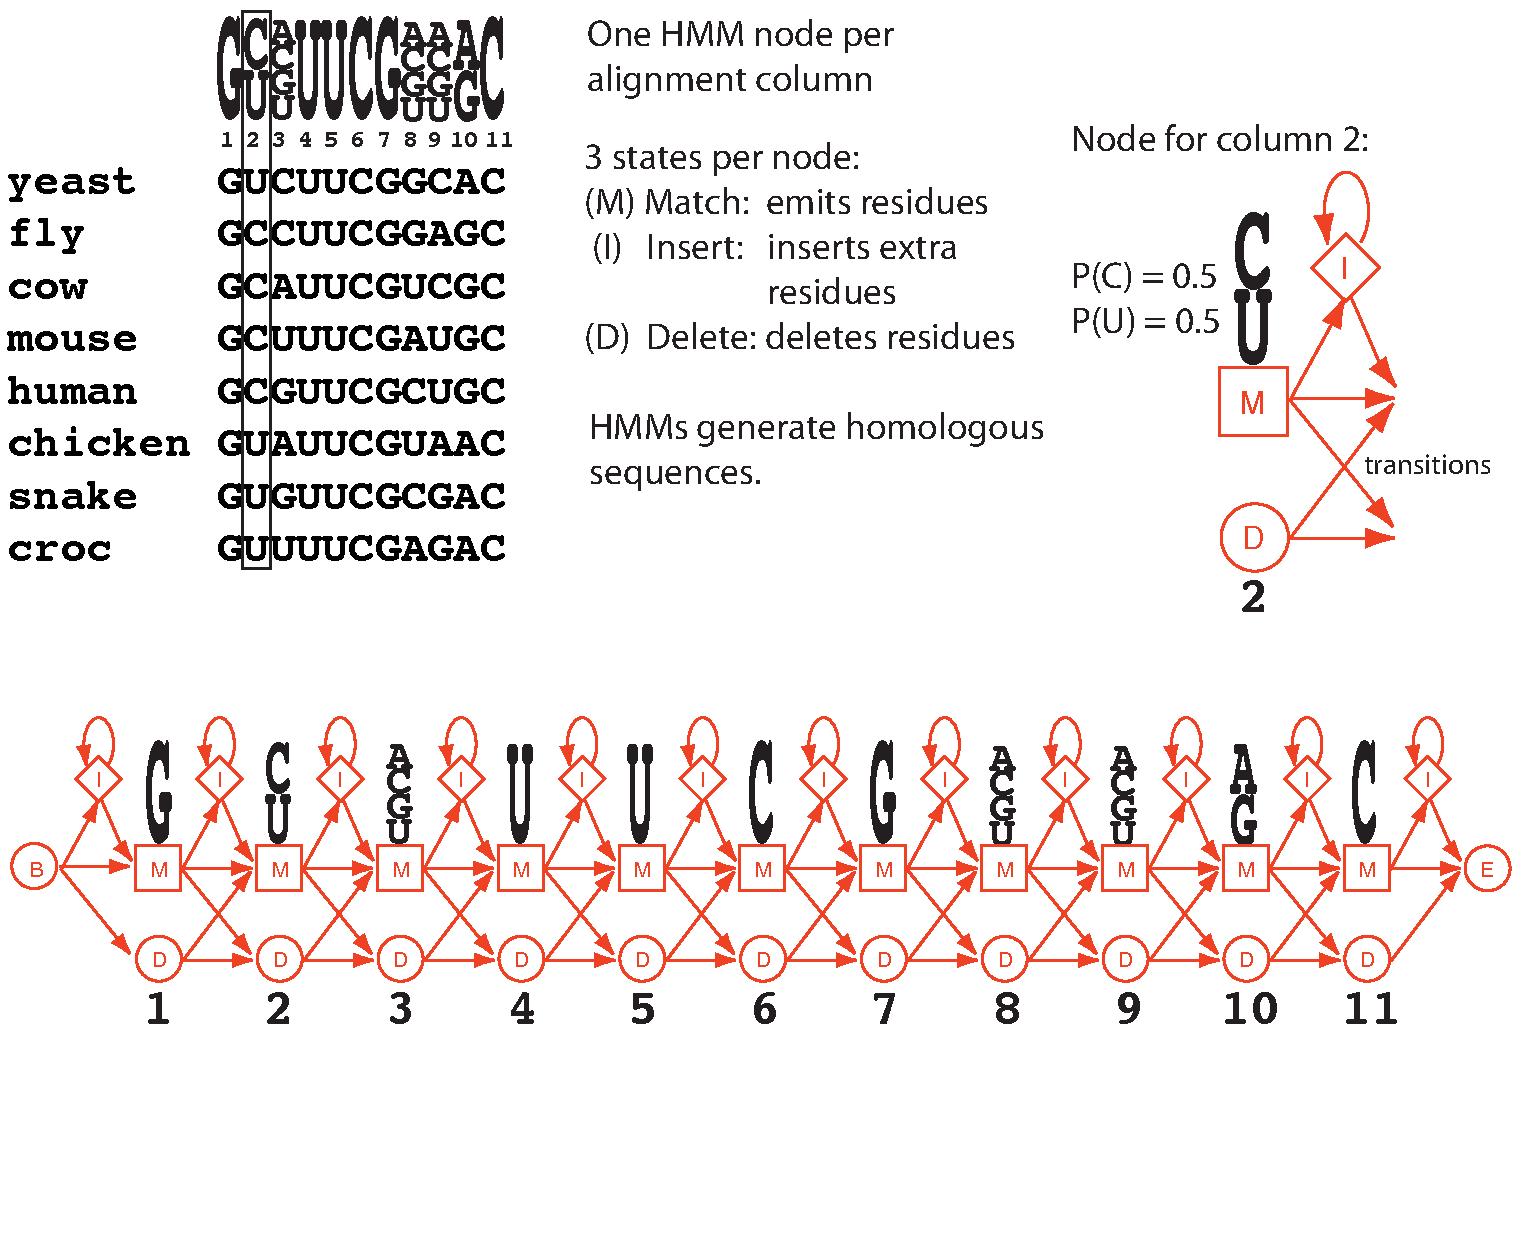
\includegraphics[height=6.625in]{figs/hmm}}

%An HMM generates ``homologous'' sequences.

\end{slide}
%%%%%%%%%%%%%%%%%%%%%%%%%%%%%%%%%%%%%%%%%%%%%%%%%%%%%%%%%%%%%%%
\begin{slide}
\begin{center}
%\textbf{profile HMMs and covariance models}
\textbf{Profile HMMs: sequence family models built from alignments}
\end{center}

\center{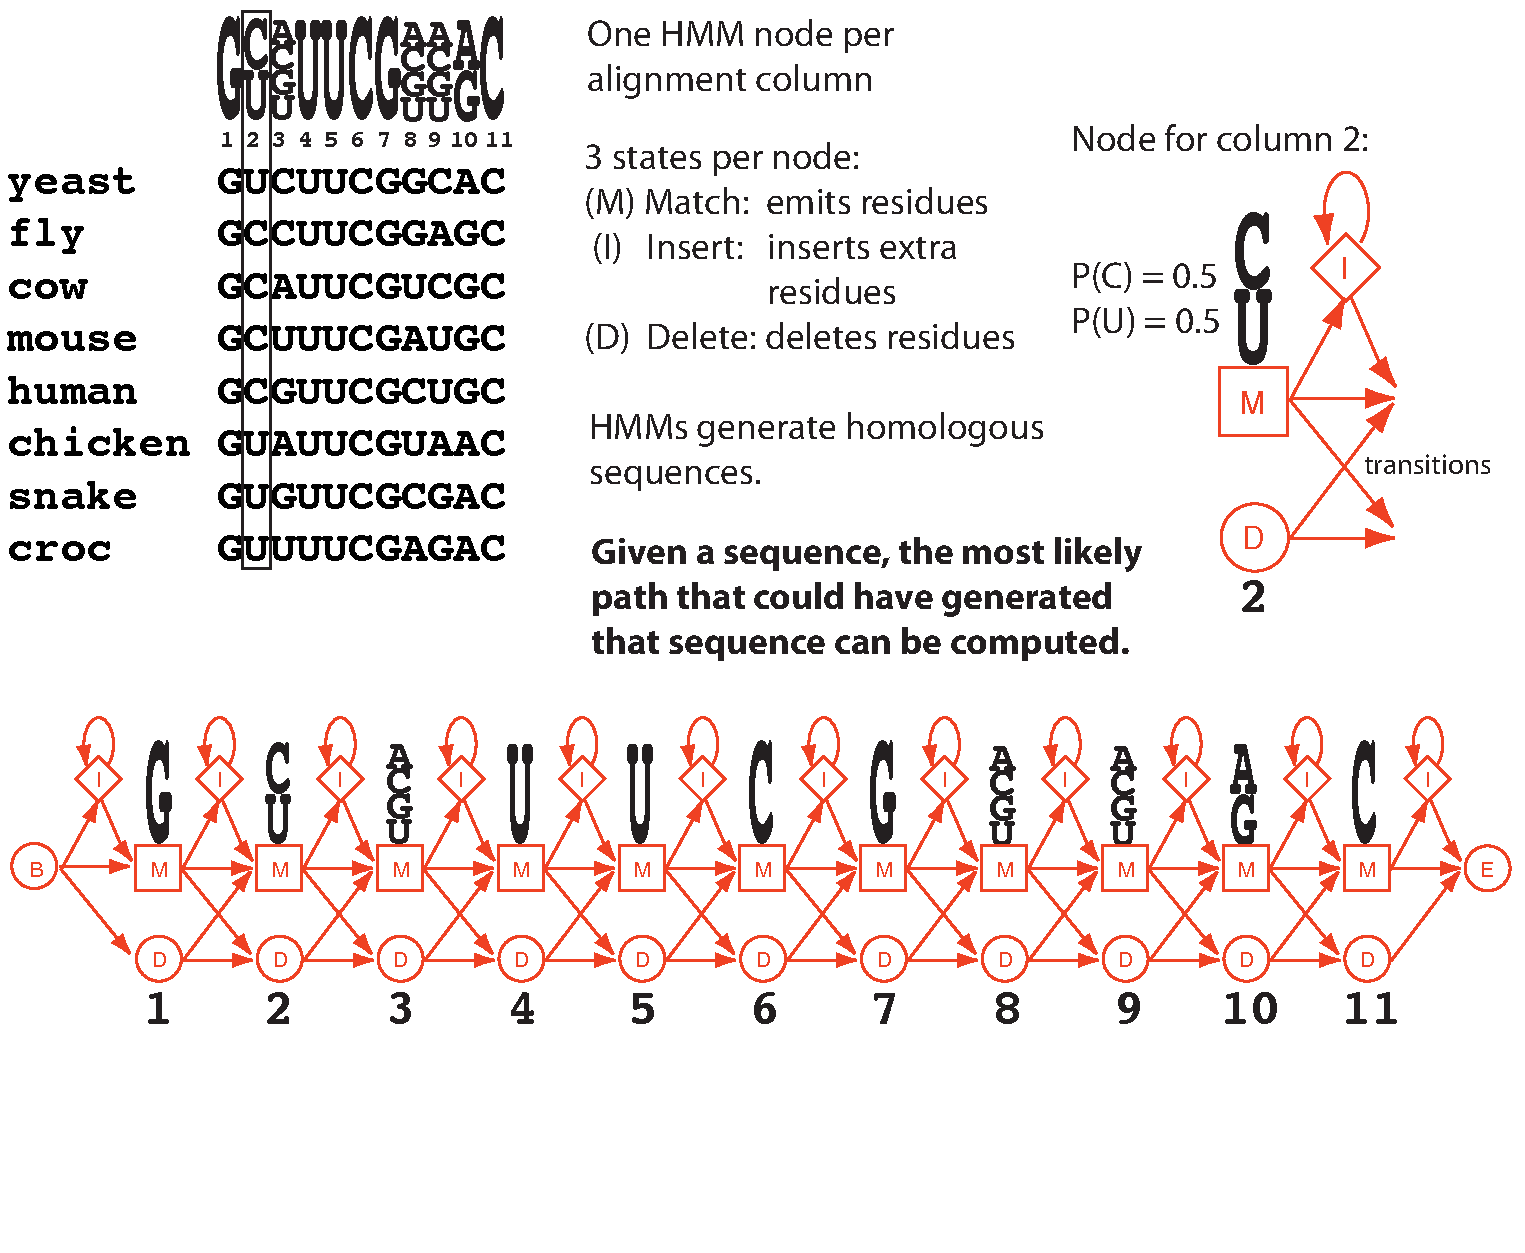
\includegraphics[height=6.625in]{figs/hmm-given}}
\end{slide}
%%%%%%%%%%%%%%%%%%%%%%%%%%%%%%%%%%%%%%%%%%%%%%%%%%%%%%%%%%%%%%%
\begin{slide}
\begin{center}
%\textbf{profile HMMs and covariance models}
\textbf{Profile HMMs: sequence family models built from alignments}
\end{center}

\center{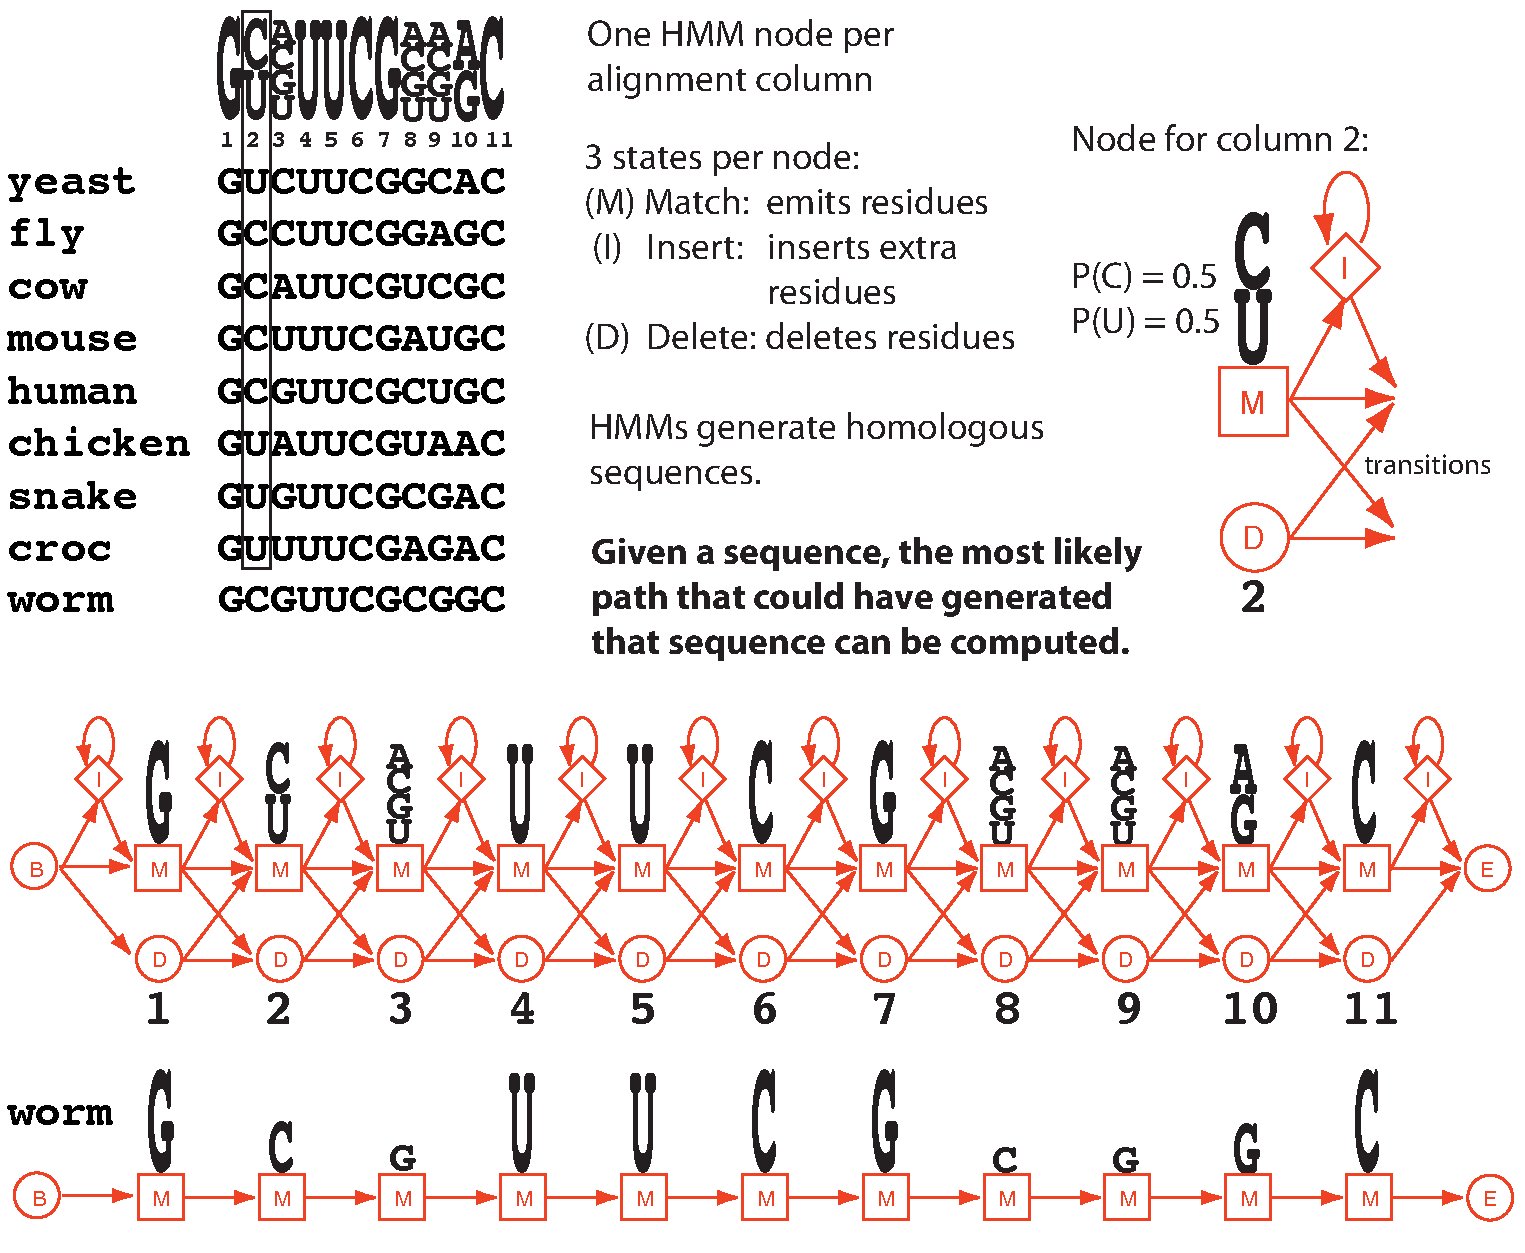
\includegraphics[height=6.625in]{figs/hmm-worm}}
\end{slide}
%%%%%%%%%%%%%%%%%%%%%%%%%%%%%%%%%%%%%%%%%%%%%%%%%%%%%%%%%%%
\begin{slide}
\begin{center}
%\textbf{profile HMMs and covariance models}
\textbf{Profile HMMs: sequence family models built from alignments}
\end{center}

\center{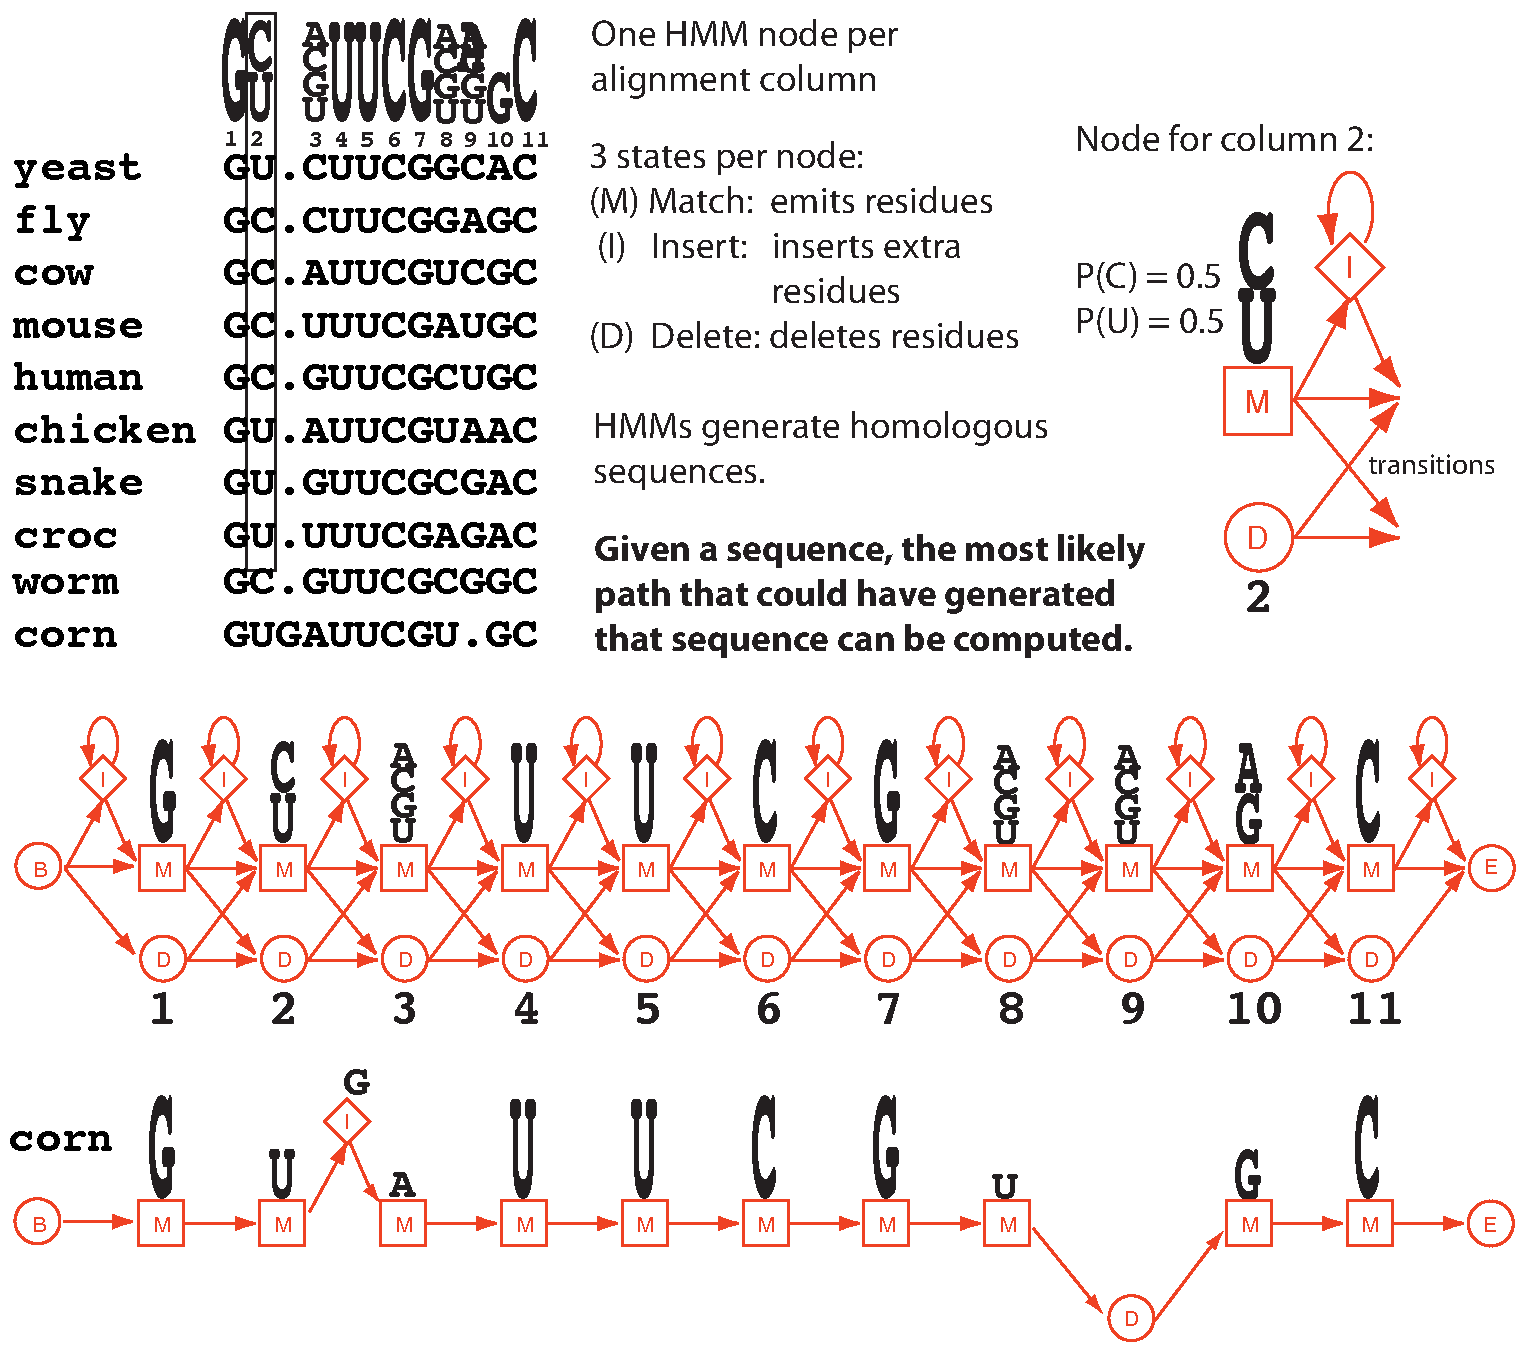
\includegraphics[height=6.625in]{figs/hmm-corn}}
\end{slide}
%%%%%%%%%%%%%%%%%%%%%%%%%%%%%%%%%%%%%%%%%%%%%%%%%%%%%%%%%%%%%%%
\begin{slide}
\begin{center}
%\textbf{profile HMMs and covariance models}
\textbf{Covariance models (CMs) are built \\ from structure-annotated alignments}
\end{center}

\center{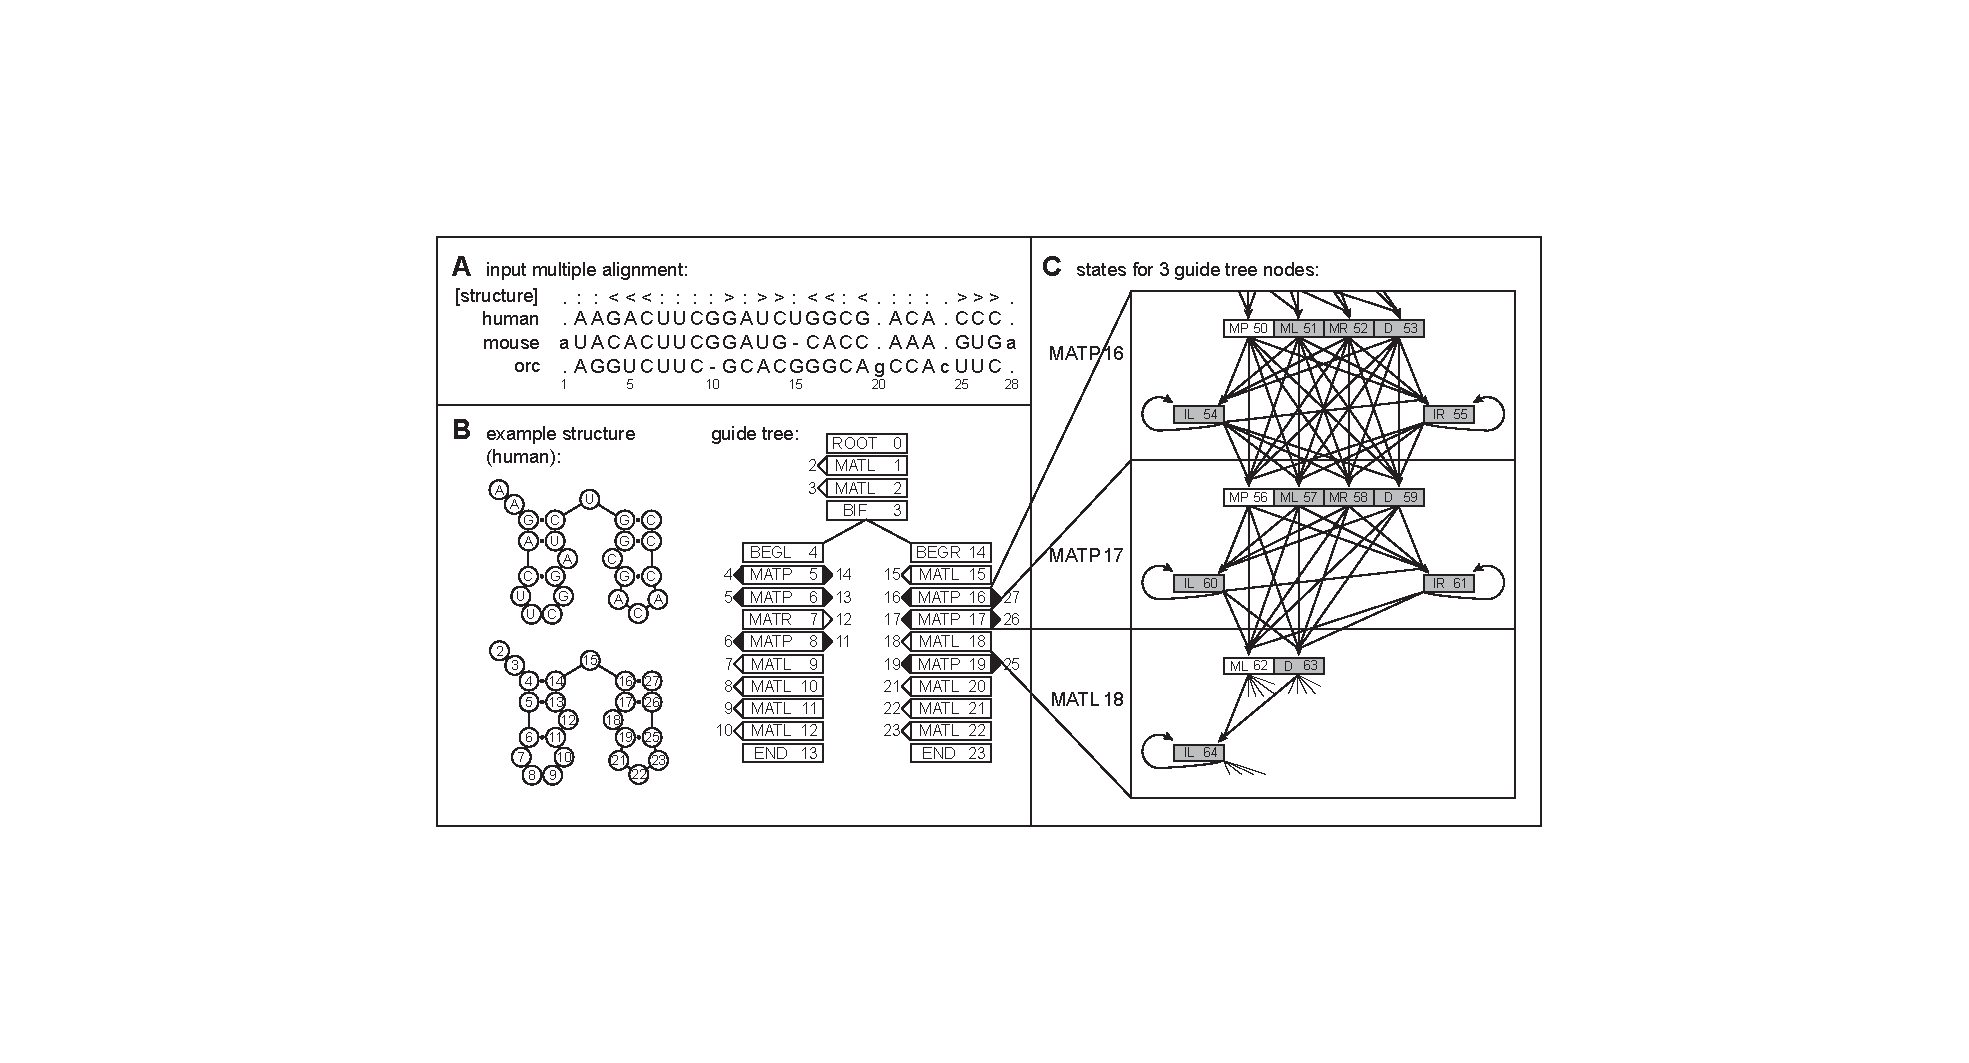
\includegraphics[width=7in]{figs/cmintro_bandcyk}}

\center{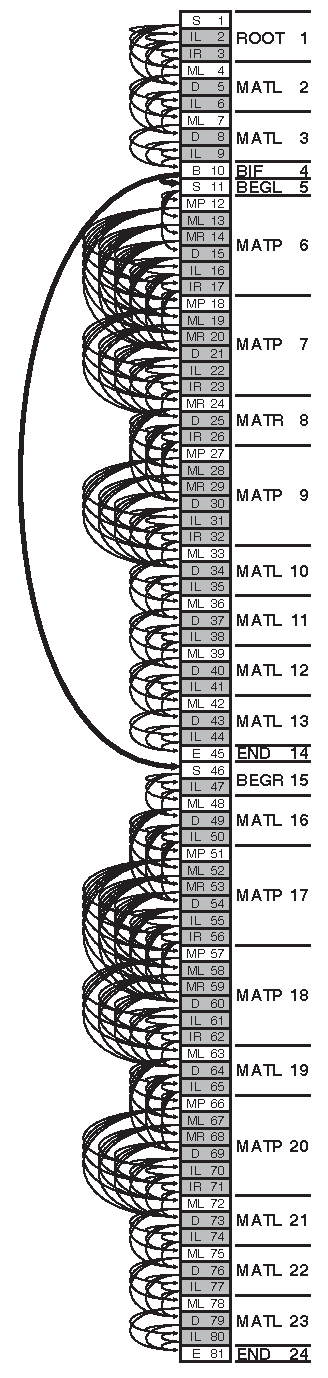
\includegraphics[width=2in,angle=270]{figs/cm-graph-small}}

\vfill

\end{slide}
%%%%%%%%%%%%%%%%%%%%%%%%%%%%%%%%%%%%%%%%%%%%%%%%%%%%%%%%%%%%%%%%%%

%%%%%%%%%%%%%%%%%%%%%%%%%%%%%%%%%%%%%%%%%%%%%%%%%%%%%%%%%%%%%%%
%%%%%%%%%%%%%%%%%%%%%%%%%%%%%%%%%%%%%%%%%%%%%%%%%%%%%%%%%%%%%%%
%%%%%%%%%%%%%%%%%%%%%%%%%%%%%%%%%%%%%%%%%%%%%%%%%%%%%%%%%%%%%%%
%%%%%%%%%%%%%%%%%%%%%%%%%%%%%%%%%%%%%%%%%%%%%%%%%%%%%%%%%%%%%%%
%%%%%%%%%%%%%%%%%%%%%%%%%%%%%%%%%%%%%%%%%%%%%%%%%%%%%%%%%%%%%%%
%%%%%%%%%%%%%%%%%%%%%%%%%%%%%%%%%%%%%%%%%%%%%%%%%%%%%%%%%%%%%%%
\begin{slide}
\begin{center}

\textbf{Infernal outperforms primary-sequence based methods on our
  benchmark (and others\footnote{Freyhult EK, Bollback JP, Gardner
    PP. Genome Res. 2007 17: 117-125.}, not shown)}

\end{center}
\medskip

\center{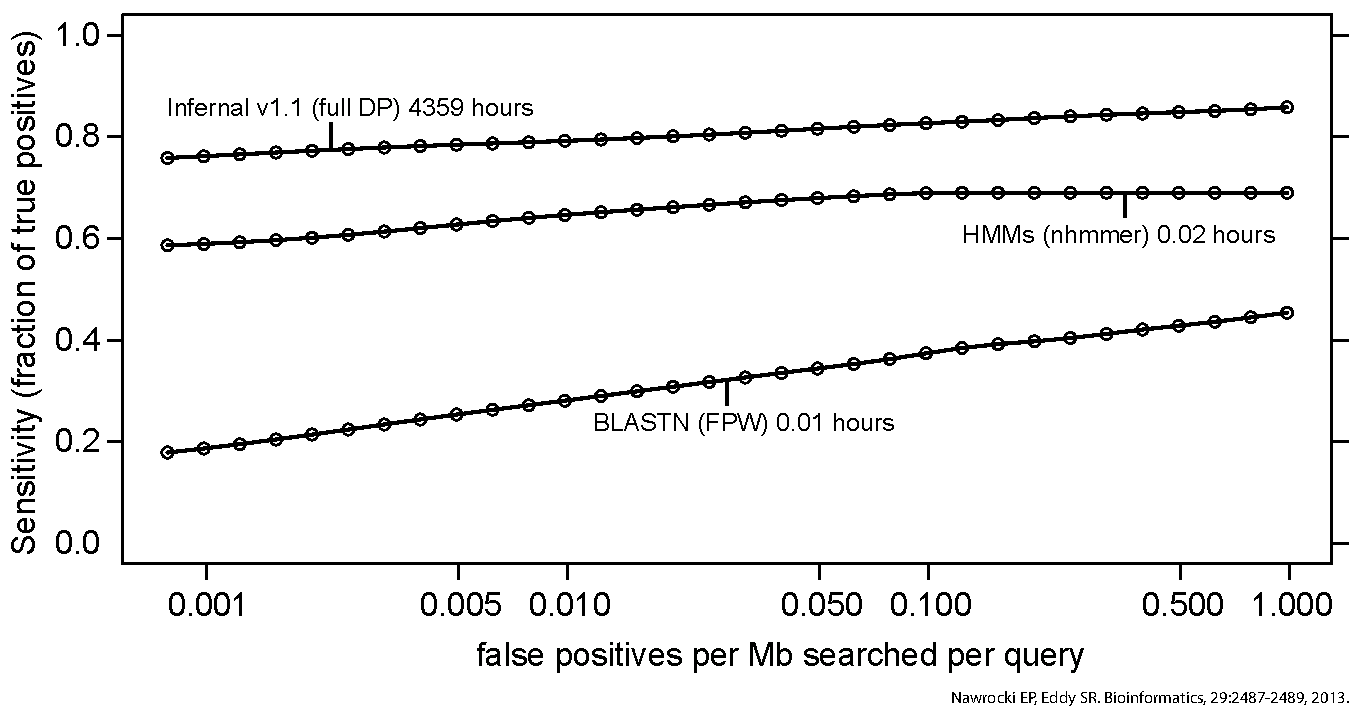
\includegraphics[width=10in]{figs/roc-talk-rcb-2014-1}}

\vfill 
\end{slide}
%%%%%%%%%%%%%%%%%%%%%%%%%%%%%%%%%%%%%%%%%%%%%%%%%%%%%%%%%%%%%%%%%%%%%%
\begin{slide}
\begin{center}
\large
\textbf{Filter target database using profile HMMs\footnote{Weinberg,
    Ruzzo, RECOMB, 243-251, 2004; Weinberg, Ruzzo, Bioinformatics,
    22(1) 35-39 2006.}}
\end{center}

\center{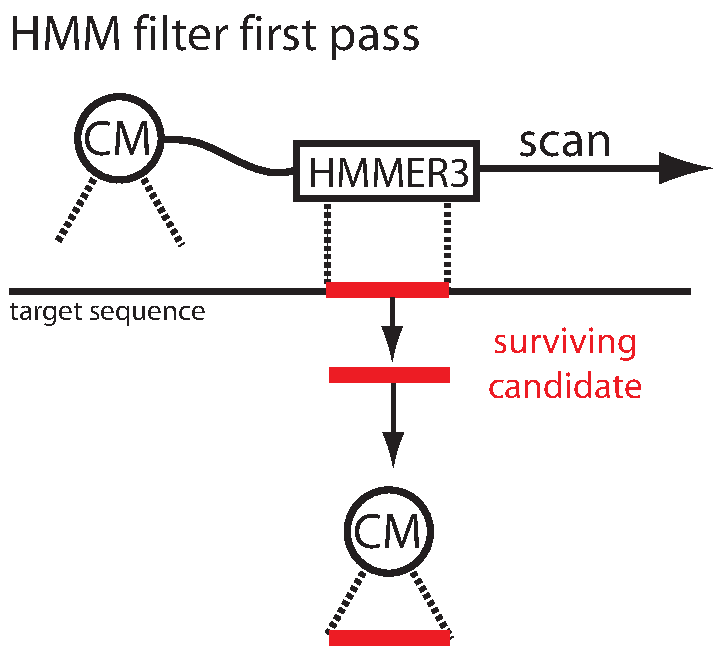
\includegraphics[height=4in]{figs/filter-2014-1}}

\vfill
\end{slide}
%%%%%%%%%%%%%%%%%%%%%%%%%%%%%%%%%%%%%%%%%%%%%%%%%%%%%%%%%%%%%%%%%%%%%%%%%%
\begin{slide}
\begin{center}
\large
\textbf{Filter target database using profile HMMs\footnote{Weinberg,
    Ruzzo, RECOMB, 243-251, 2004; Weinberg, Ruzzo, Bioinformatics,
    22(1) 35-39 2006.}}
\end{center}

\center{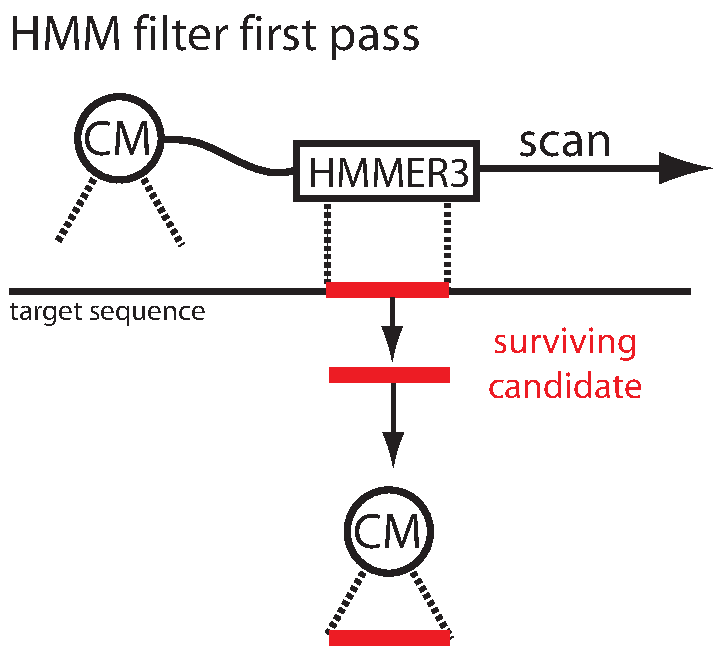
\includegraphics[height=4in]{figs/filter-2014-1}}

\begin{itemize}
\item Even if we filter out 99\% of the database (for up to 100X
  acceleration), searches will still be too slow.
\item CM step needs to be accelerated. 
\end{itemize}

\vfill
\end{slide}
%%%%%%%%%%%%%%%%%%%%%%%%%%%%%%%%%%%%%%%%%%%%%%%%%%%%%%%%%%%%%%%%%%%%%%%%%%
%\begin{slide}
%\begin{center}
%
%\textbf{Accelerating CM alignment step 1: \\ align sequence with HMM}
%
%\includegraphics[height=6in]{figs/hmm_alignment2_layer2}
%\end{center}
%
%\vfill
%\end{slide}
%%%%%%%%%%%%%%%%%%%%%%%%%%%%%%%%%%%%%
%%%%%%%%%%%%%%%%%%%%%%%%%%%%%%%%%%%%%%%%%%%%%%%%%%%%%%%%%%%%%%%%%%%%%%%%%%
\begin{slide}
\begin{center}

%\textbf{Accelerating CM alignment step 2: \\ HMM posterior decoding to
%  get confidence estimates}
\textbf{Accelerating CM alignment step 1: \\ HMM posterior decoding to
  get confidence estimates}

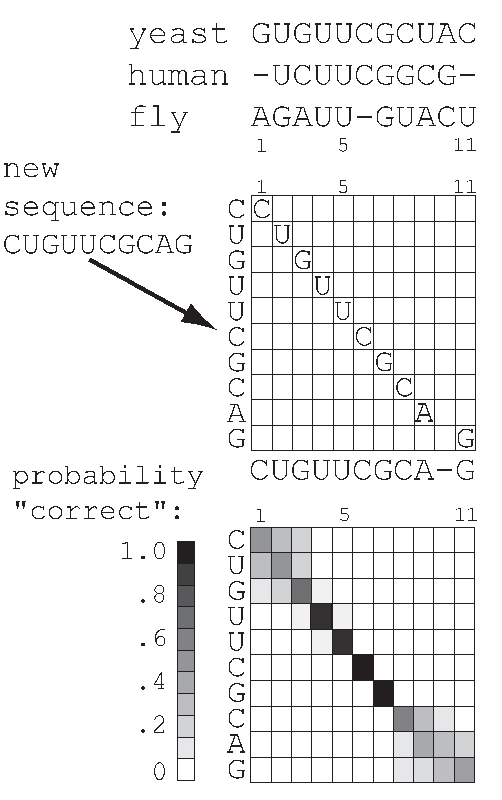
\includegraphics[height=6in]{figs/hmm_alignment2_layer3}
\end{center}

\vfill
\end{slide}
%%%%%%%%%%%%%%%%%%%%%%%%%%%%%%%%%%%%%
\begin{slide}
\begin{center}

\textbf{Accelerating CM alignment step 2: \\ use HMM alignment
  confidence to constrain CM alignment\footnote{M. P. Brown. Proc. Int. Conf. ISMB, 8:57–66, 2000.}}
\end{center}
\medskip
\small
%\begin{itemize}
%\item
%\textbf{main idea:} eliminate potential alignments the HMM tells us are very improbable
%\end{itemize}
\begin{center}
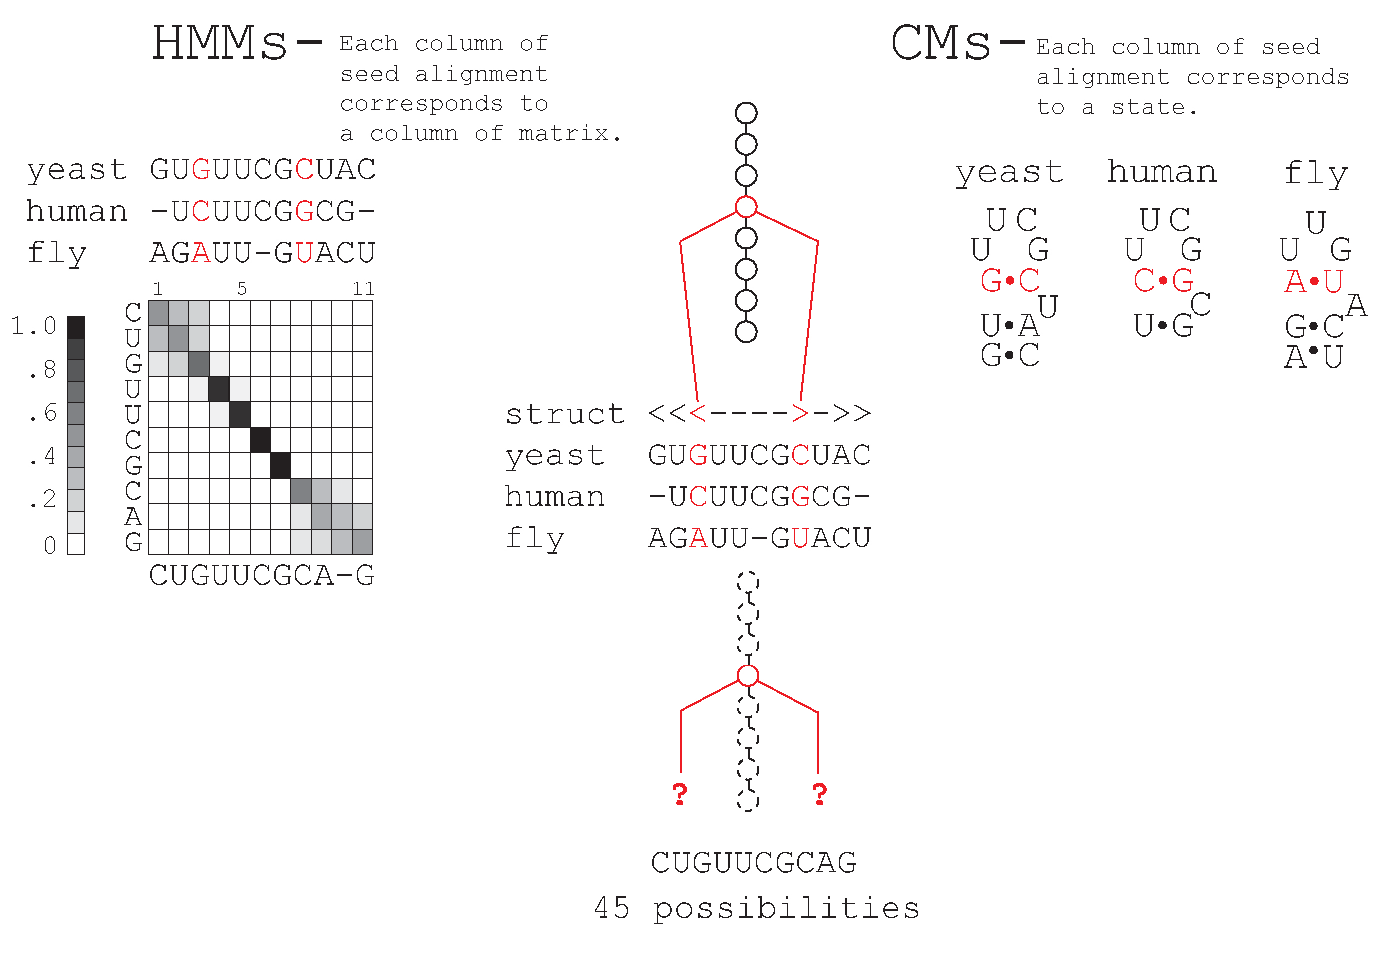
\includegraphics[width=8in]{figs/post_hmm_to_cm_map2_layer14}
\end{center}
\vfill
\end{slide}
%%%%%%%%%%%%%%%%%%%%%%%%%%%%%%%%%%%%%%%%%%%%%%%%%%%%%%%%%%%%%%%%%%%%%%
\begin{slide}
\begin{center}

\textbf{Accelerating CM alignment step 2: \\ use HMM alignment
  confidence to constrain CM alignment\footnote{M. P. Brown. Proc. Int. Conf. ISMB, 8:57–66, 2000.}}
\end{center}
\medskip
\small
%\begin{itemize}
%\item
%\textbf{main idea:} eliminate potential alignments the HMM tells us are very improbable
%\end{itemize}
\begin{center}
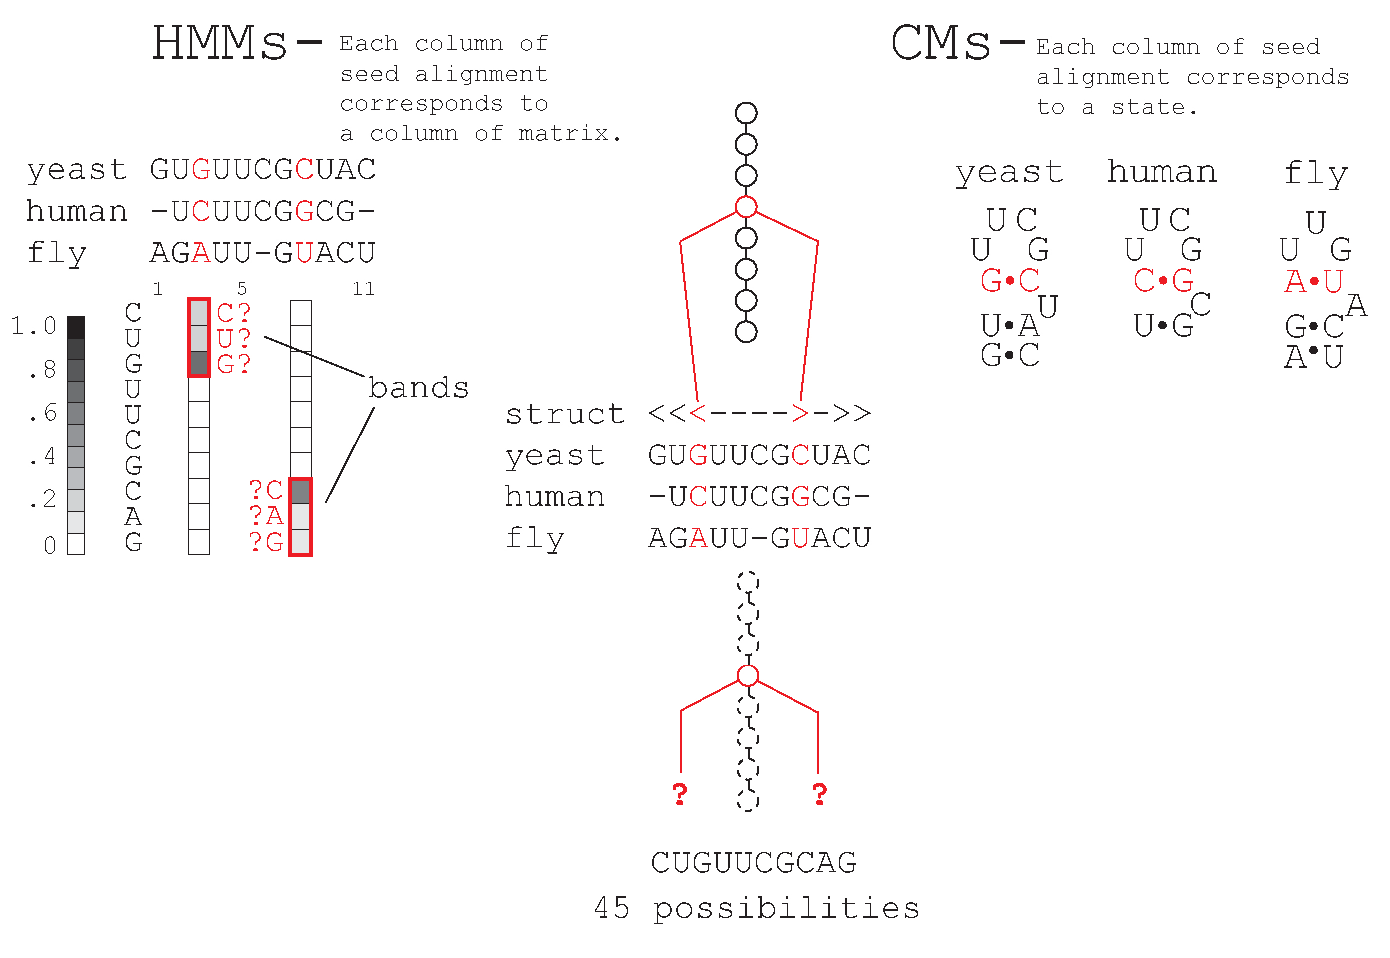
\includegraphics[width=8in]{figs/post_hmm_to_cm_map2_layer15}
\end{center}
\vfill
\end{slide}
%%%%%%%%%%%%%%%%%%%%%%%%%%%%%%%%%%%%%%%%%%%%%%%%%%%%%%%%%%%%%%%%%%%%%%%%%%
\begin{slide}
\begin{center}

\textbf{Accelerating CM alignment step 3: \\ use HMM alignment
  confidence to constrain CM alignment\footnote{M. P. Brown. Proc. Int. Conf. ISMB, 8:57–66, 2000.}}
\end{center}
\medskip
\small
%\begin{itemize}
%\item
%\textbf{main idea:} eliminate potential alignments the HMM tells us are very improbable
%\end{itemize}
\begin{center}
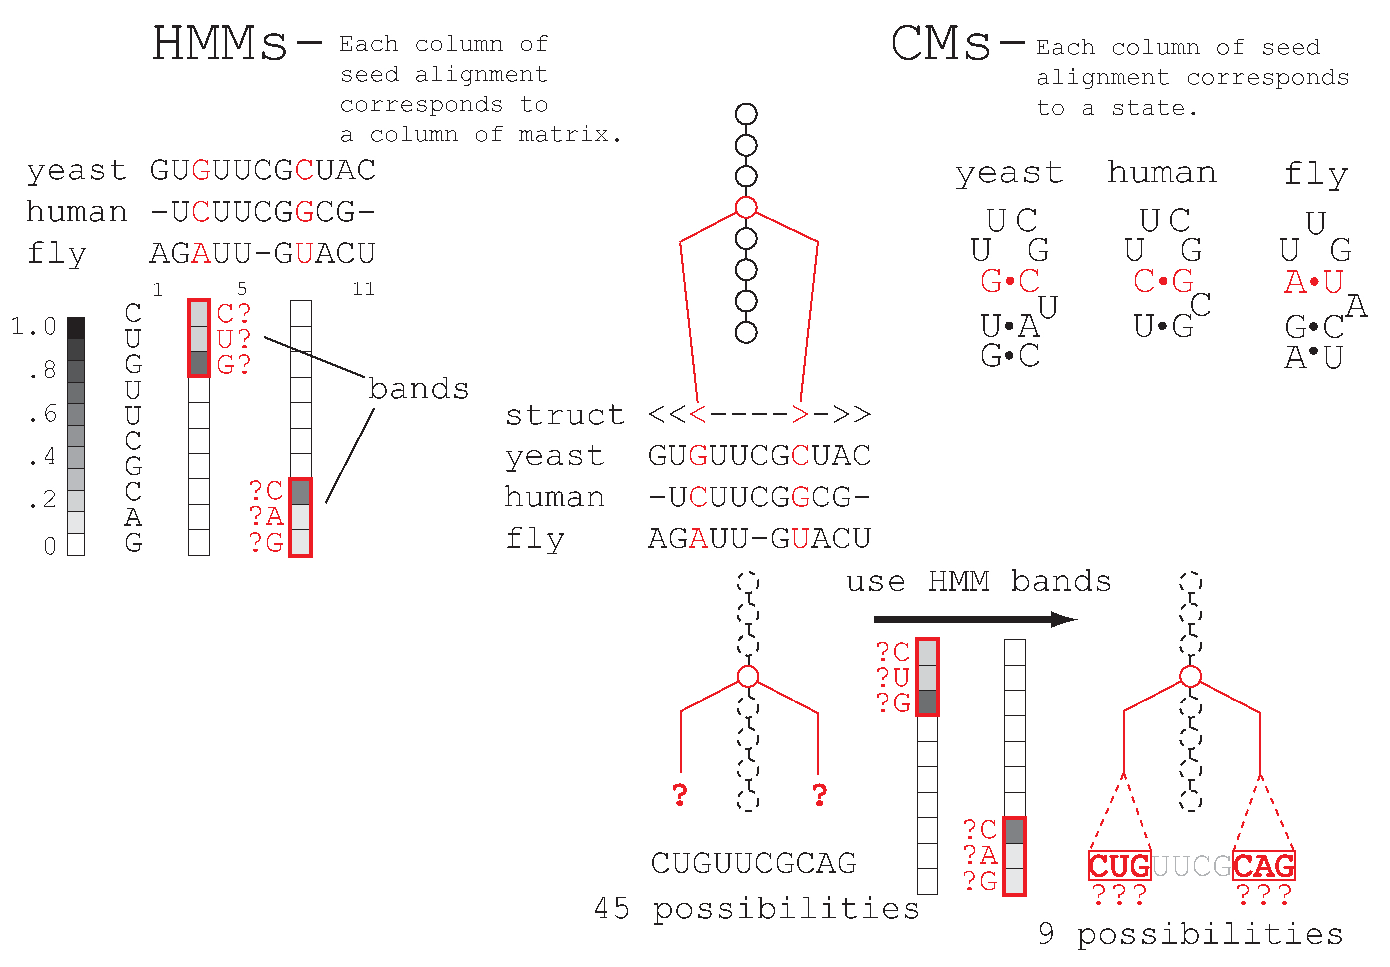
\includegraphics[width=8in]{figs/post_hmm_to_cm_map2_layer16}
\end{center}
\vfill
\end{slide}
%%%%%%%%%%%%%%%%%%%%%%%%%%%%%%%%%%%%%%%%%%%%%%%%%%%%%%%%%%%%%%%%%%%%%%
\begin{slide}
\center{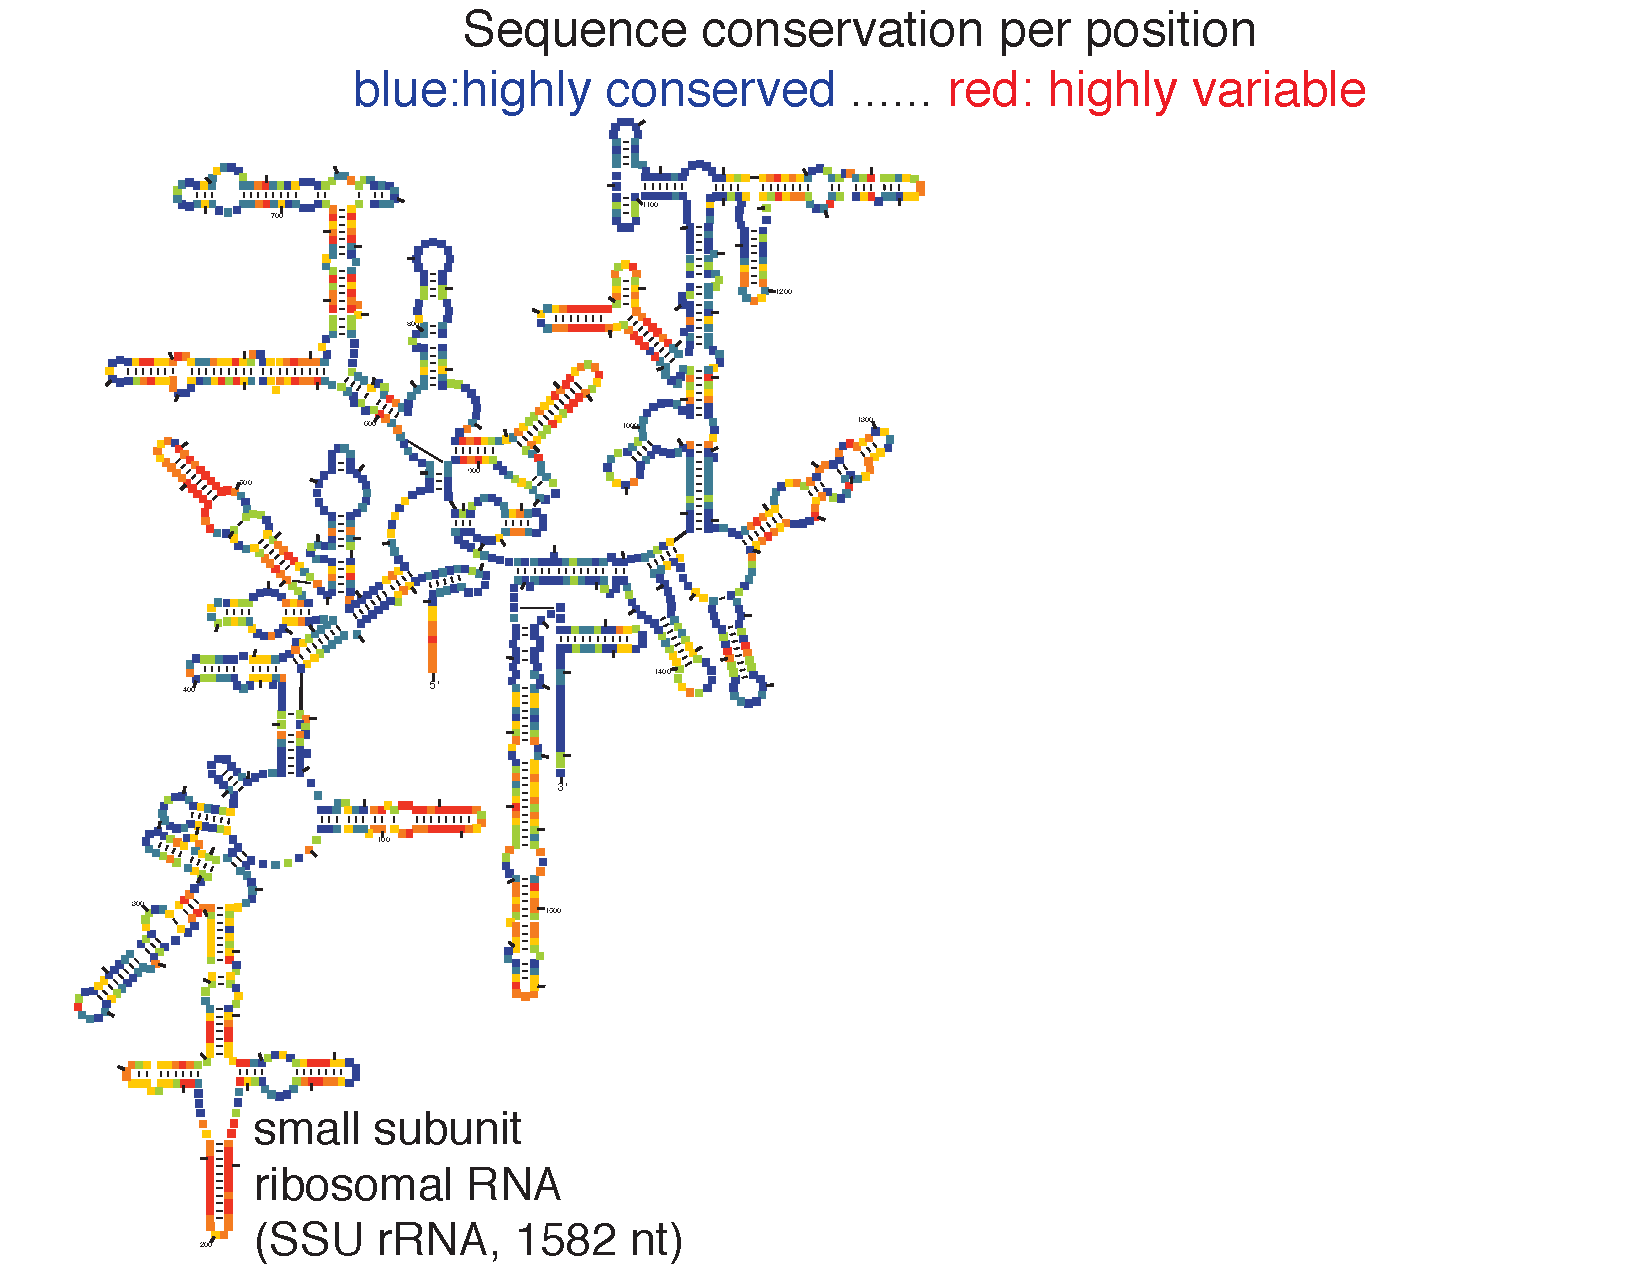
\includegraphics[width=10.5in]{figs/16s-5s-trna-info-16sonly}}
\end{slide}
%%%%%%%%%%%%%%%%%%%%%%%%%%%%%%%%%%%%%%%%%%%%%%%%%%%%%%%%%%%%%%%%%%%%%%
\begin{slide}
\center{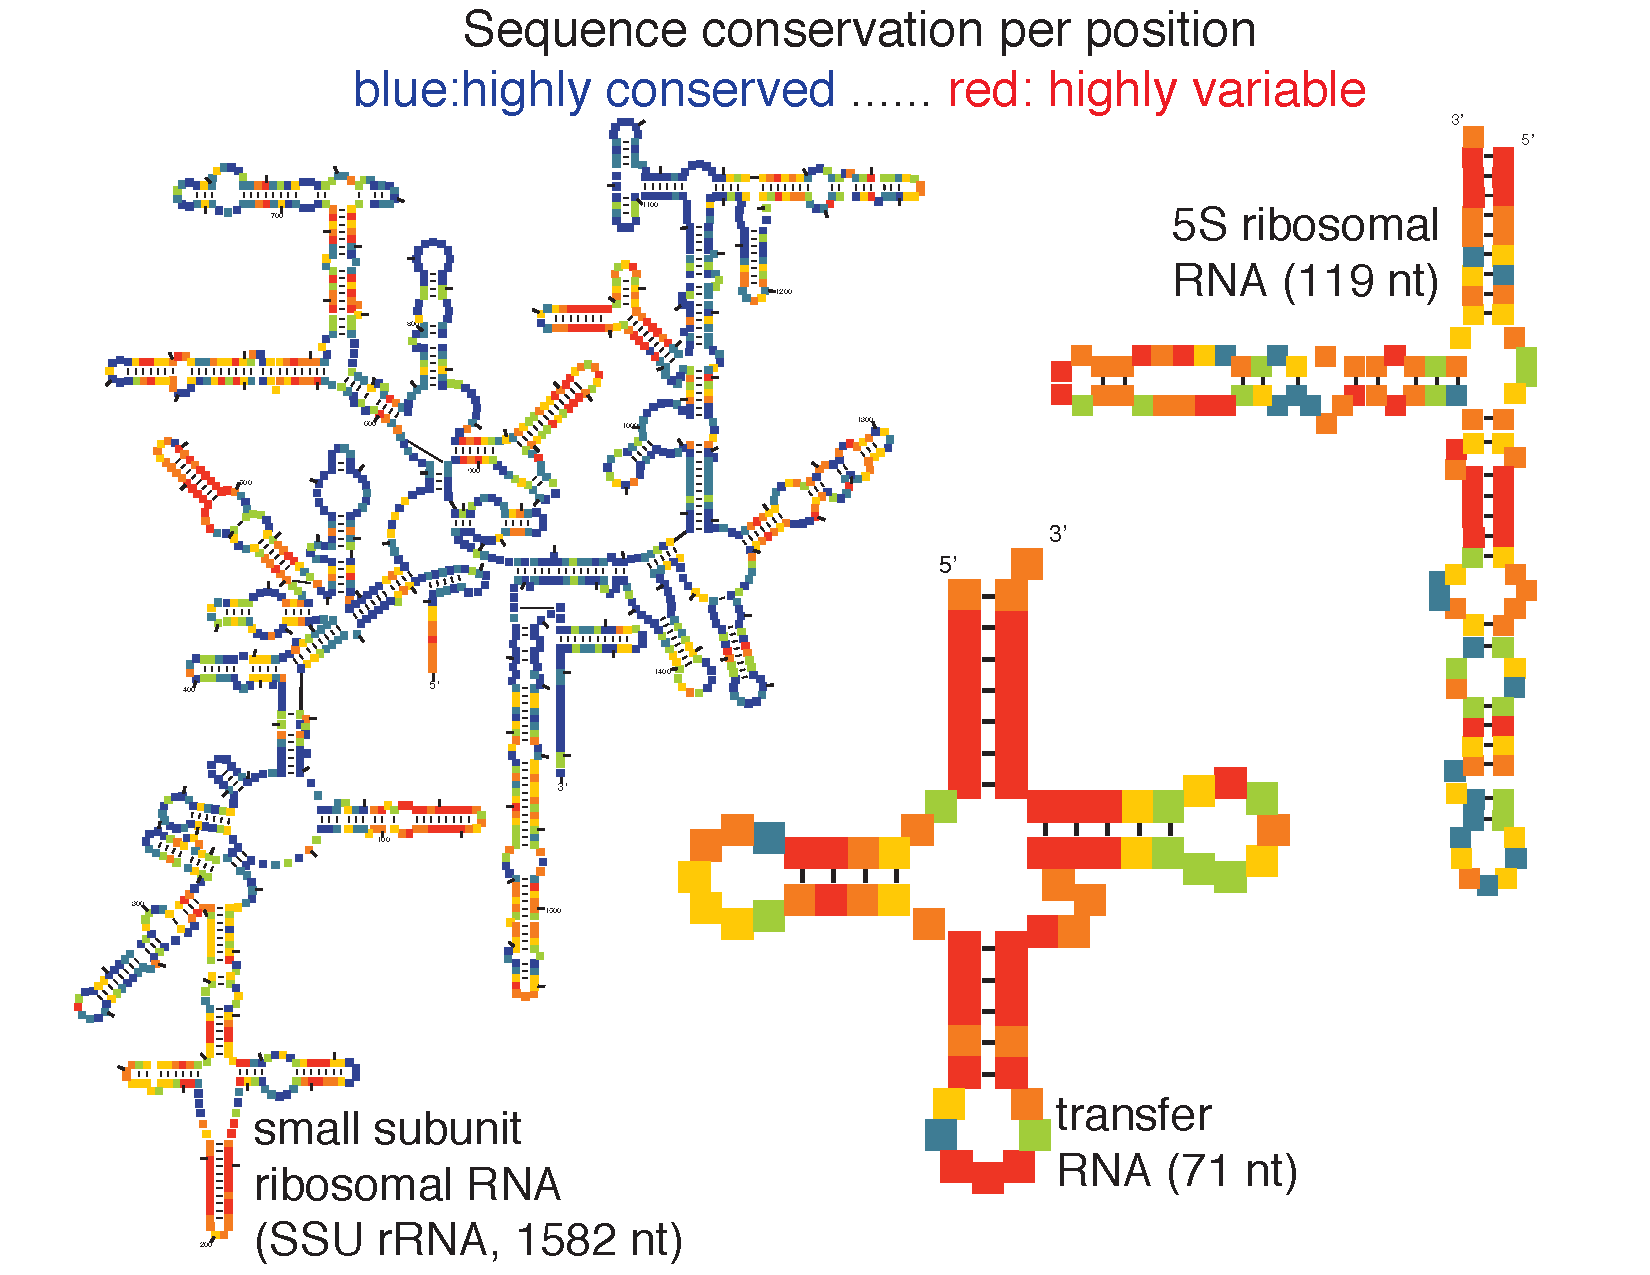
\includegraphics[width=10.5in]{figs/16s-5s-trna-info}}
\end{slide}
%%%%%%%%%%%%%%%%%%%%%%%%%%%%%%%%%%%%%%%%%%%%%%%%%%%%%%%%%%%%%%%%%%%%
\begin{slide}
\begin{center}
\large
\textbf{Use HMMs as filters and to constrain CM alignment}
\end{center}

\center{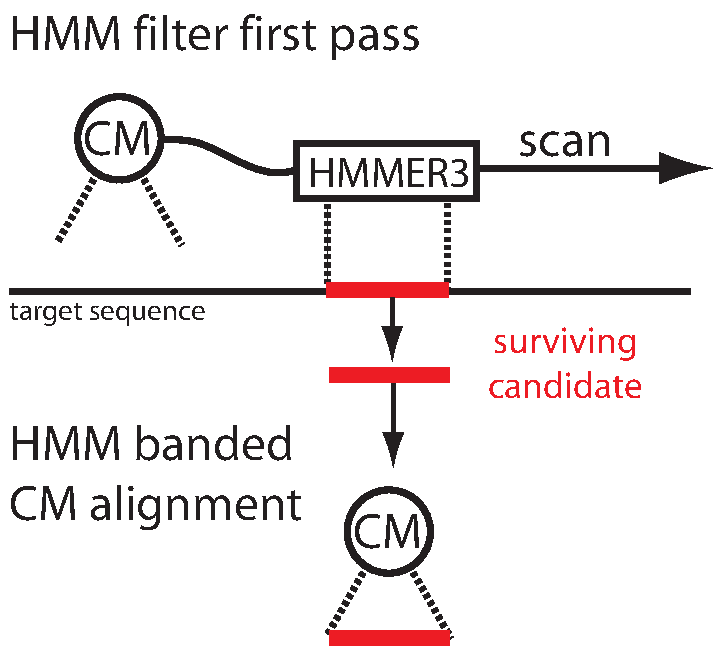
\includegraphics[height=5in]{figs/filter-2014-2}}

\vfill
\end{slide}
%%%%%%%%%%%%%%%%%%%%%%%%%%%%%%%%%%%%%%%%%%%%%%%%%%%%%%%%%%%%%%%%%%%%%%%%%%
\begin{slide}
\begin{center}

\textbf{HMM-based acceleration makes Infernal 10,000 times faster}

\end{center}
\medskip

\center{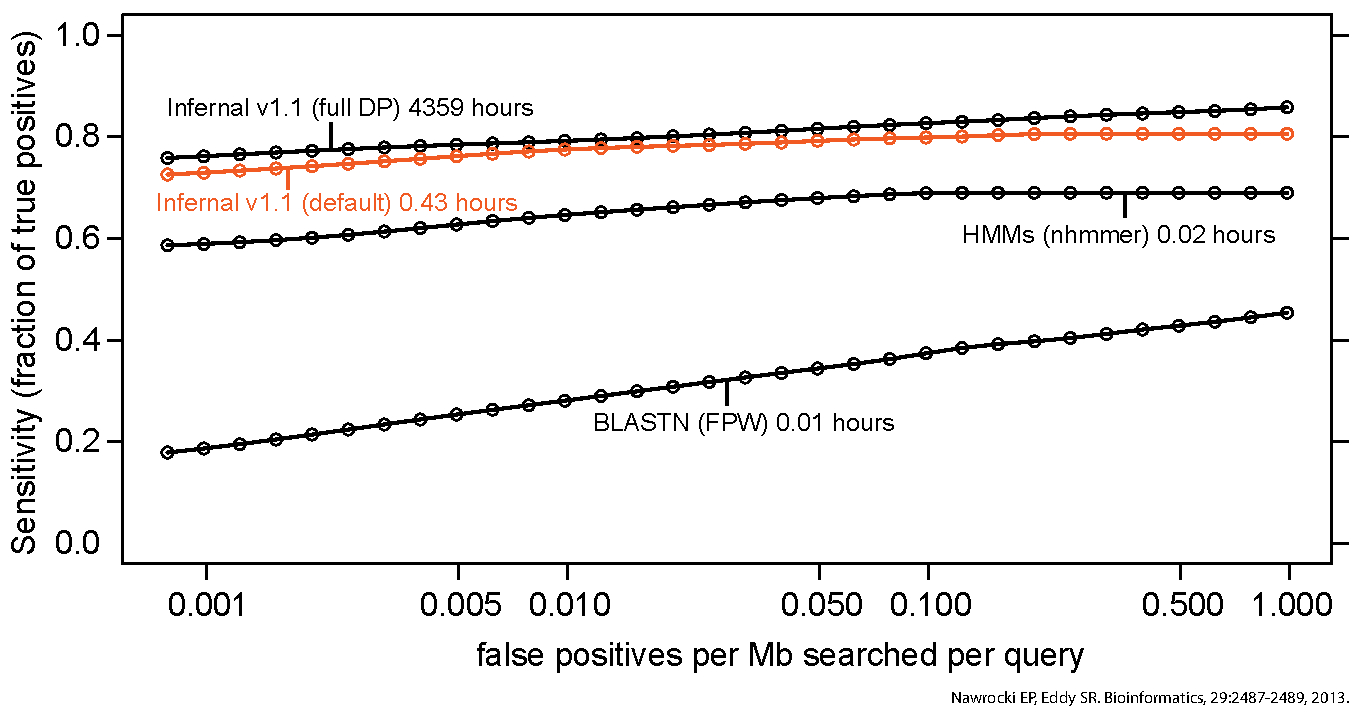
\includegraphics[width=10in]{figs/roc-talk-rcb-2014-2}}

\vfill 
\end{slide}


%%%%%%%%%%%%%%%%%%%%%%%%%%%%%%%%%%%%%%%%%%%%%%%%%%%%%%%%%%%%%%%%%%%%%%
\begin{slide}
\begin{center}

\textbf{Rfam used BLAST filters from 2003 to 2012}

\end{center}

\begin{itemize}
\item Rfam includes $>$ 2000 RNA families, each represented by an
  alignment, CM and set of predicted homologs in a large database (Rfamseq).
\end{itemize}

\center{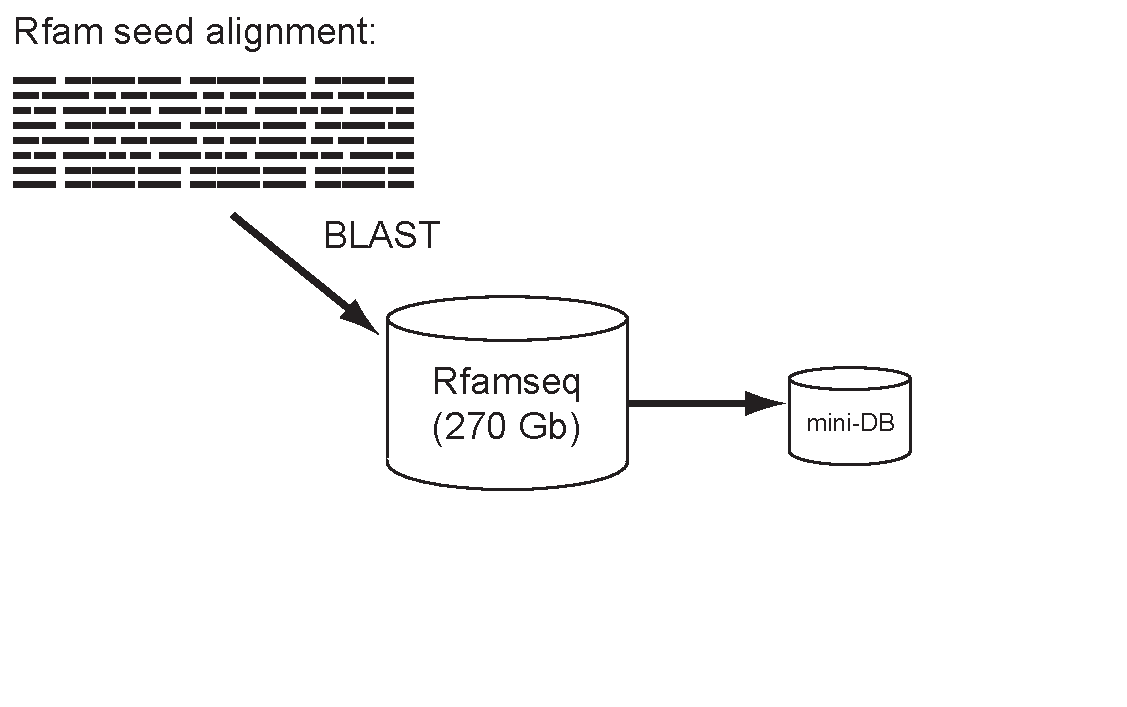
\includegraphics[width=8in]{figs/rfam-search-1}}

\vfill
\end{slide}
%%%%%%%%%%%%%%%%%%%%%%%%%%%%%%%%%%%%%%%%%%%%%%%%%%%%%%%%%%%%%%%%%%%%%%
\begin{slide}
\begin{center}

\textbf{Rfam used BLAST filters from 2003 to 2012}

\end{center}

\begin{itemize}
\item Rfam includes $>$ 2000 RNA families, each represented by an
  alignment, CM and set of predicted homologs in a large database (Rfamseq).
\end{itemize}

\center{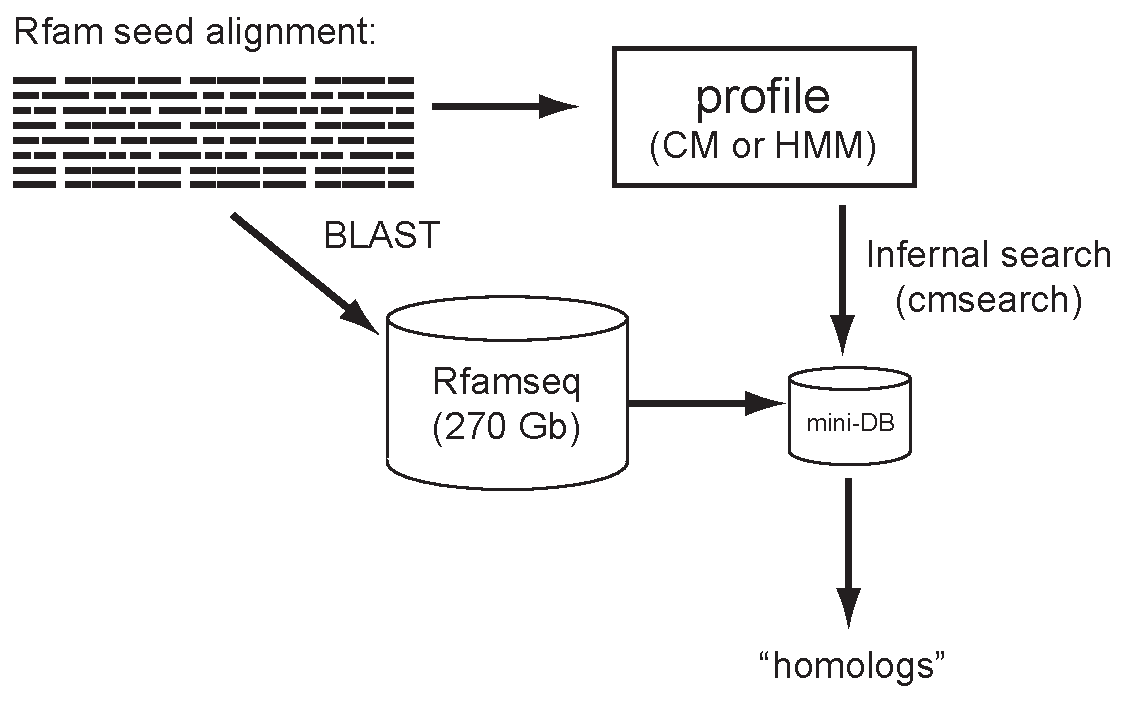
\includegraphics[width=8in]{figs/rfam-search-2}}

\vfill
\end{slide}
%%%%%%%%%%%%%%%%%%%%%%%%%%%%%%%%%%%%%%%%%%%%%%%%%%%%%%%%%%%%%%%%%%%%%%
\begin{slide}
\begin{center}

\textbf{Rfam 12.0 (2014)\footnote{Nawrocki, Burge et. al, NAR 43:D130-D137, 2015.}, 
first release without BLAST filtering}
\end{center}

\center{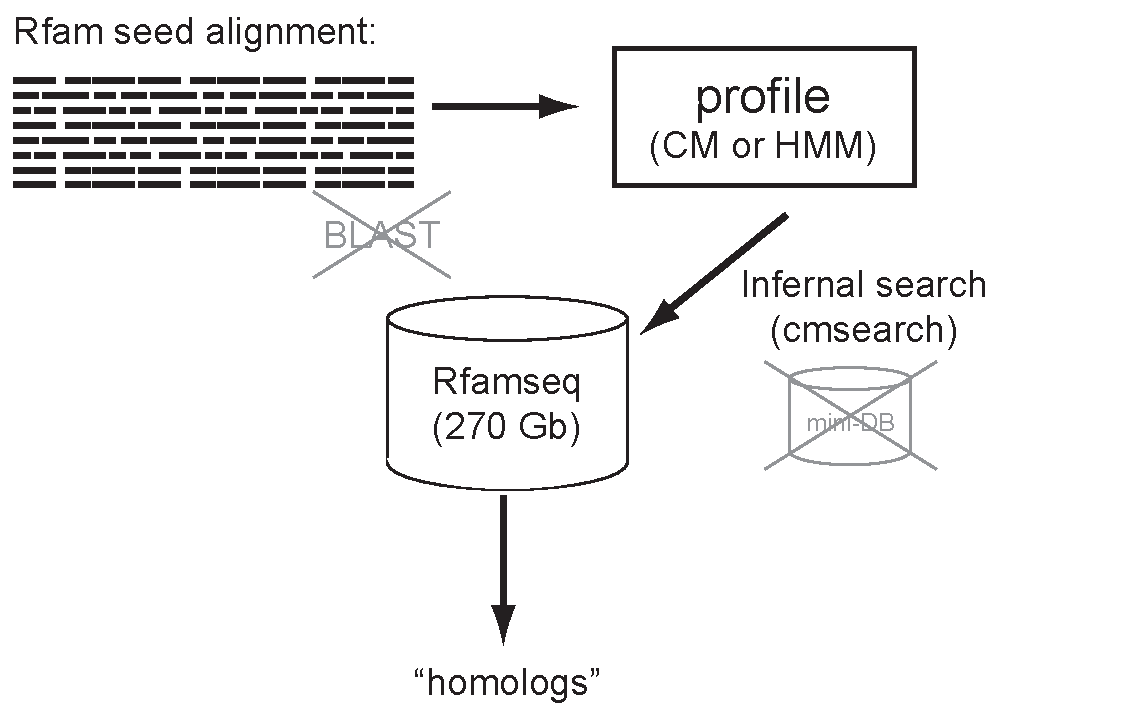
\includegraphics[width=8in]{figs/rfam-search-3}}

%\begin{center}
%\small
%Search results against Rfamseq for 200 random families:
%\begin{tabular}{l|rrr}
%strategy                   & time (h) & \# hits & \# unique hits \\ \hline
%Old (BLAST + Infernal 1.0) & 4069.8   &  179681 & 53 \\
%New (Infernal 1.1)         & 4222.2   &  201814 & 22312 \\
%\end{tabular}
%\end{center}

\vfill
\end{slide}
%%%%%%%%%%%%%%%%%%%%%%%%%%%%%%%%%%%%%%%%%%%%%%%%%%%%%%%%%%%%%%%%%%%%%%
\begin{slide}
\begin{center}

\textbf{Rfam 12.0 (2014)\footnote{Nawrocki, Burge et. al, NAR 43:D130-D137, 2015.}, 
first release without BLAST filtering}

\end{center}

\begin{center}
Search results against Rfamseq for 200 random families:

\medskip

\begin{tabular}{l|r|r|r}
strategy                   & time (h) & \# hits & \# unique hits \\ \hline
& & & \\
Old (BLAST + Infernal 1.0) & 4069.8   &  179,681 & 53 \\
& & & \\
New (Infernal 1.1)         & 4222.2   &  201,814 & 22,312 \\
\end{tabular}
\end{center}

\vfill
\end{slide}
%%%%%%%%%%%%%%%%%%%%%%%%%%%%%%%%%%%%%%%%%%%%%%%%%%%%%%%%%%%%%%%%%%%%%%
%\begin{slide}
%\begin{center}
%\small
%\end{center}
%
%\center{\includegraphics[width=10.5in]{figs/rfam-nar-table1-published}}
%
%\vfill
%\end{slide}
%%%%%%%%%%%%%%%%%%%%%%%%%%%%%%%%%%%%%%%%%%%%%%%%%%%%%%%%%%%%%%%%%%%%%%
\begin{slide}
\begin{center}
\textbf{Infernal 1.1 finds 11,000 new group I intron candidates}
\end{center}

%\center{\includegraphics[width=10.5in]{figs/rfam-nar-table1-published-gp1i-yellow}}
\center{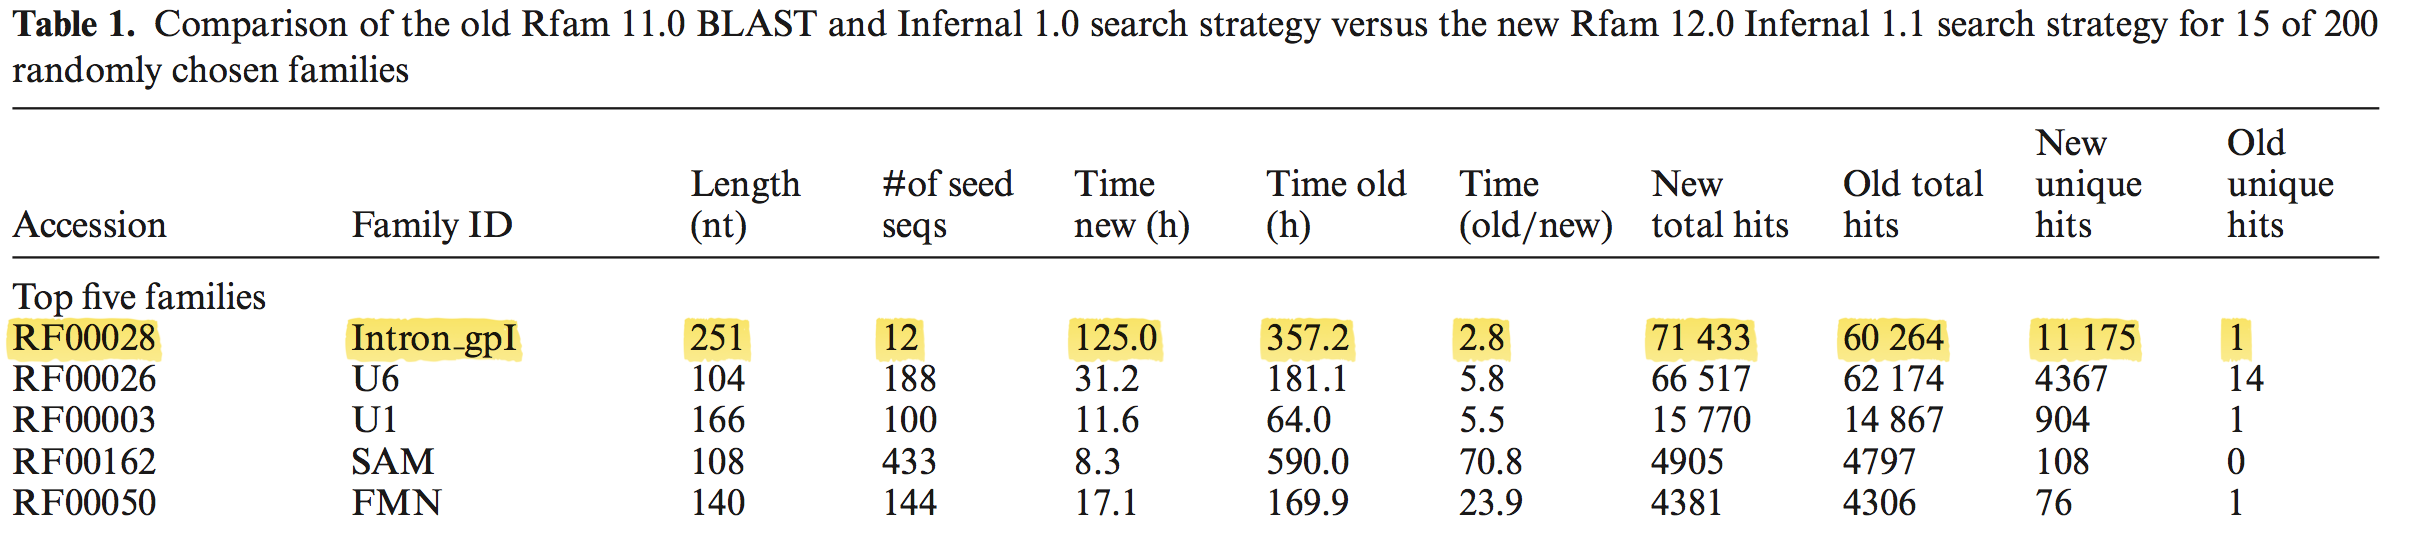
\includegraphics[width=10.5in]{figs/rfam-nar-table1-published-gp1i-yellow-top5only}}

\vfill
\vfill
\small
\flushleft{Nawrocki, Burge et. al, NAR 43:D130-D137, 2015.} 
\end{slide}
%%%%%%%%%%%%%%%%%%%%%%%%%%%%%%%%%%%%%%%%%%%%%%%%%%%%%%%%%%%%%%%%%%%%%%%%%
\begin{slide}
\begin{center}
\textbf{It is now easier to use Rfam/Infernal to annotate your own
  datasets.} \\

\small
\begin{itemize}
\item A bacterial genome takes about 30 minutes for all 2450 models.

\item Michael DiCuccio's group is working on adding
  Rfam/Infernal to the GPIPE pipeline.
\end{itemize}

\end{center}

%\center{\includegraphics[width=10.5in]{figs/rfam-nar-table2-published}}
%\center{\includegraphics[width=10.5in]{figs/rfam-nar-table2-bac-yellow-yescaption}}
\center{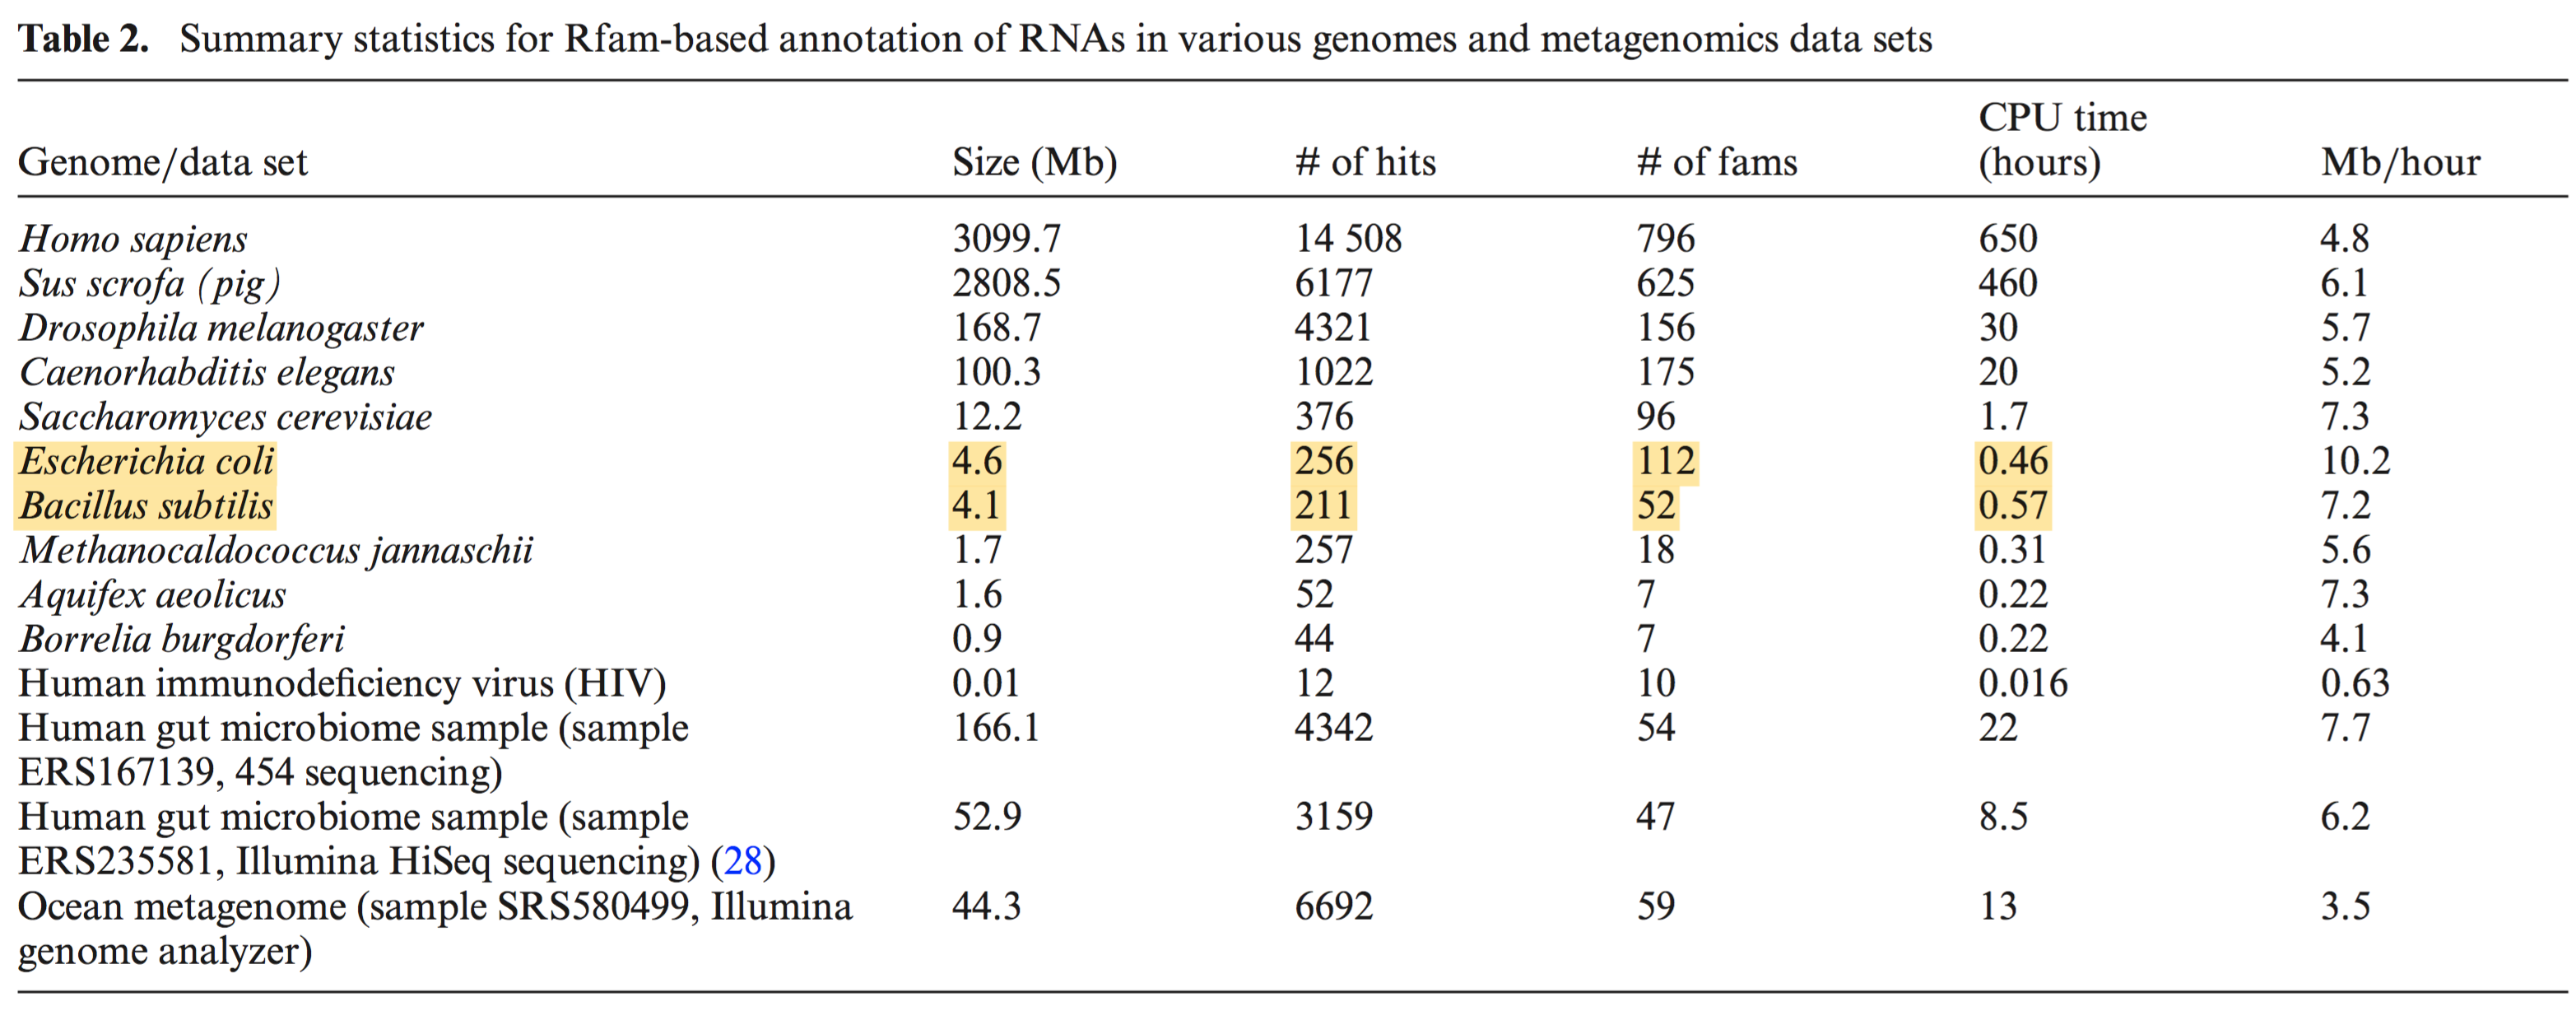
\includegraphics[width=10.5in]{figs/rfam-nar-table2-bac-yellow-nocaption}}

\vfill
\small
\flushleft{Nawrocki, Burge et. al, NAR 43:D130-D137, 2015.} 
\end{slide}
%%%%%%%%%%%%%%%%%%%%%%%%%%%%%%%%%%%%%%%%%%%%%%%%%%%%%%%%%%%%%%%%%%%%%%%%%%
\begin{slide}

\large
\begin{center}
\large{\textbf{Acknowledgements}} \\

\vspace{0.5in}

\textbf{Alejandro Sch\"{a}ffer} \\
\textbf{David Landsman} \\
\textbf{David Lipman}

\vspace{0.5in}

\normalsize
%\begin{tabular}{llllll}
%Sean Eddy           & & & & & Michael Brent \\ 
%Elena Rivas         & & & & & Jeremy Buhler \\
%Tom Jones           & & & & & Justin Fay \\
%Diana Kolbe         & & & & & Jeff Gordon \\
%Seolkyoung Jung     & & & & & Rob Mitra \\
%Sergi Castellano    & & & & & Gary Stormo \\
%Fred Davis          & & & & & \\
%Lee Henry           & & & & & \\
%Michael Farrar      & & & & & \\
%Travis Wheeler      & & & & & \\
\begin{tabular}{l|l}
\textbf{Janelia} & \textbf{EBI (Rfam)} \\ \hline
{\bf Sean Eddy}     & {\bf Alex Bateman} \\
Elena Rivas         & {\bf Rob Finn} \\
Travis Wheeler      & {\bf Sarah Burge} \\ 
{\bf Tom Jones}     & {\bf Evan Floden} \\
Diana Kolbe         & John Tate \\
Seolkyoung Jung     & Jen Daub \\
Rob Finn            & \\
Jody Clements       & \\
Fred Davis          & \\
Lee Henry           & \\
Michael Farrar      & \\
\end{tabular}

%\includegraphics[height=3in]{figs/jfrc-banner1}

\end{center}

\vfill
\end{slide}
%%%%%%%%%%%%%%%%%%%%%%%%%%%%%%%%%%%%%%%%%%%%%%%%%%%%%%%%%%%%%%%
\begin{slide}
\begin{center}
\textbf{Is the added complexity worth it? \\
  RMARK: a challenging \underline{internal} RNA homology search
  benchmark}

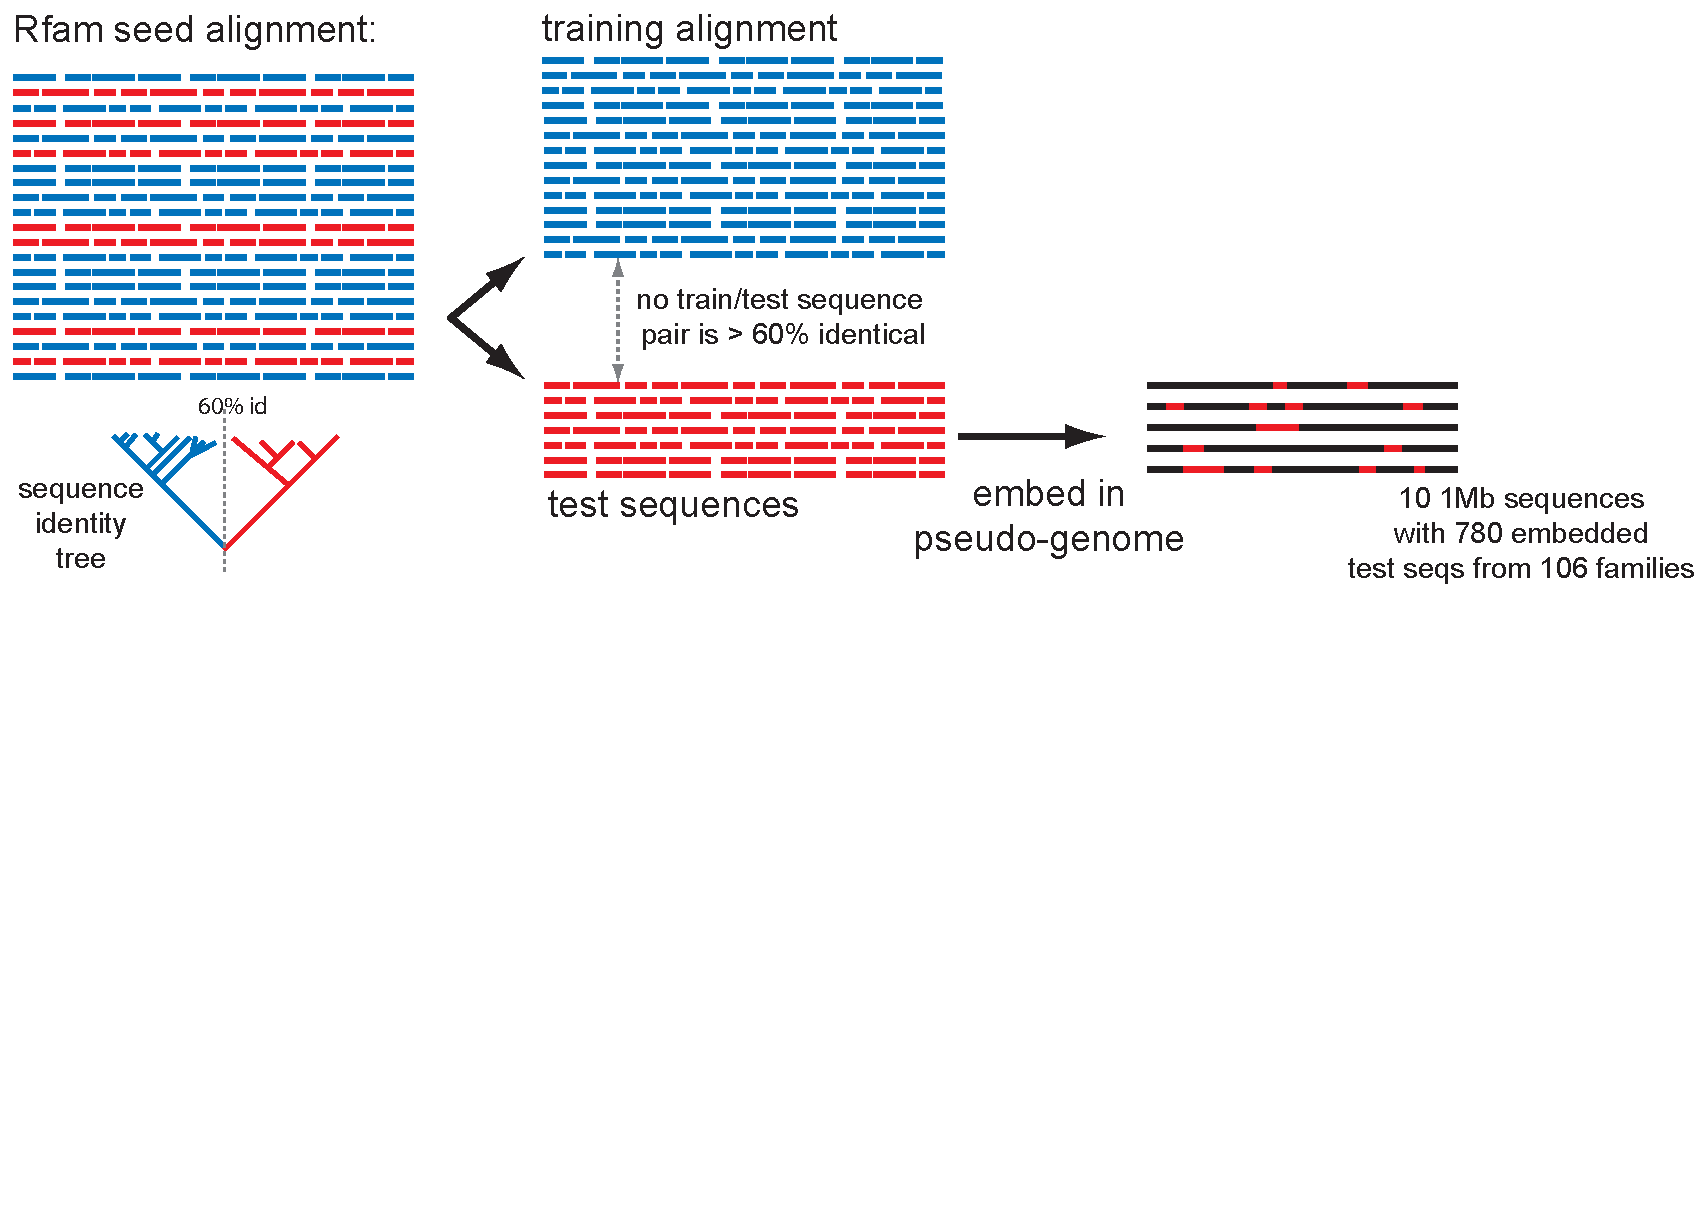
\includegraphics[width=10in]{figs/rmark-tree-1}
\end{center}

\vfill
\end{slide}
%%%%%%%%%%%%%%%%%%%%%%%%%%%%%%%%%%%%%%%%%%%%%%%%%%%%%%%%%%%%%%%%%%%%%%
\begin{slide}
\begin{center}
\textbf{Is the added complexity worth it? \\
  RMARK: a challenging \underline{internal} RNA homology search
  benchmark}

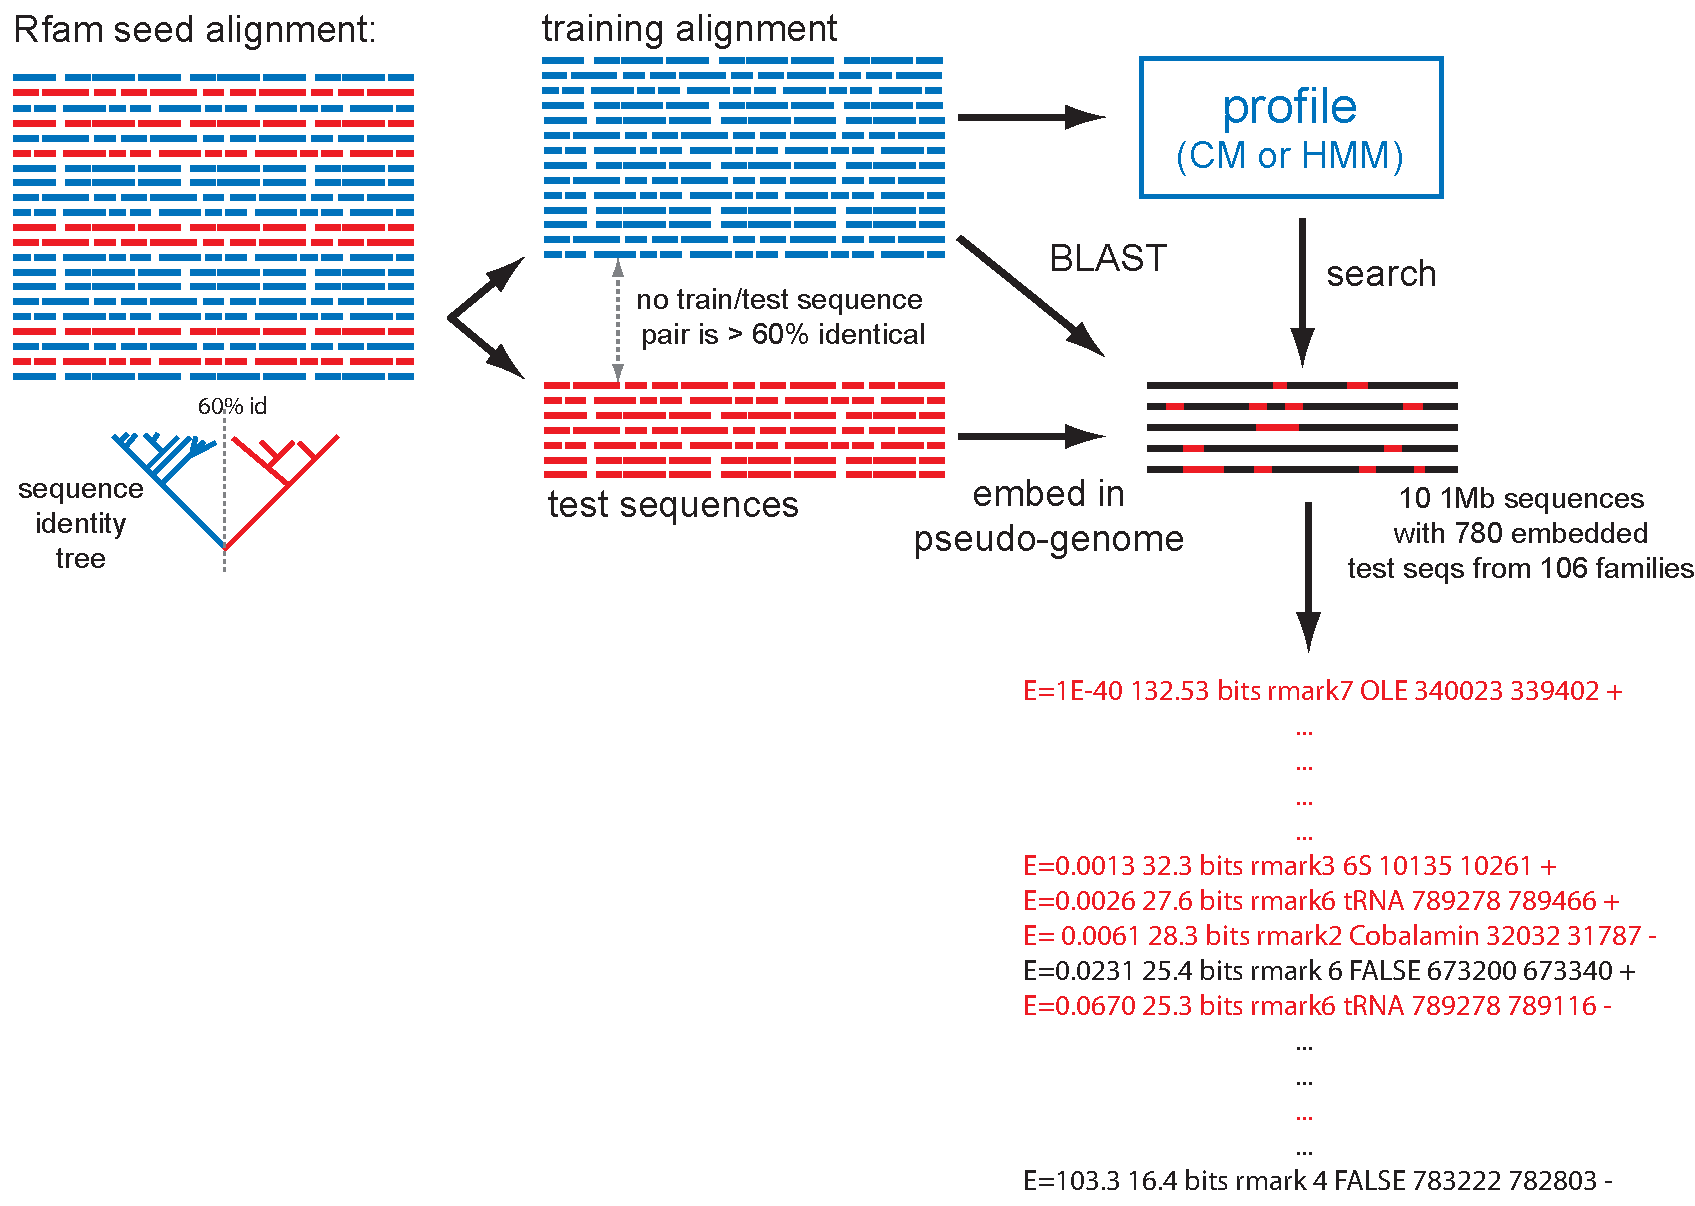
\includegraphics[width=10in]{figs/rmark-tree-2}
\end{center}

\vfill
\end{slide}
%%%%%%%%%%%%%%%%%%%%%%%%%%%%%%%%%%%%%%%%%%%%%%%%%%%%%%%%%%%%%%%%%%%%%%
%%%%%%%%%%%%%%%%%%%%%%%%%%%%%%%%%%%%%%%%%%%%%%%%%%%%%%%%%%%%%%%%%%%%%%
\begin{slide}
\begin{center}
\textbf{Applications of CMs}
\end{center}

\small
\begin{itemize}
\item homology search/alignment: Infernal,
  COVE, Rfam\footnote{E. P. Nawrocki,
    S. W. Burge et. al.
%    , A. Bateman, J. Daub, R. Y. Eberhardt, S. R. Eddy,
%    E. W. Floden, P. P. Gardner, T. A. Jones, J. Tate,
%    R. D. Finn. 
    NAR, 43:D130-D137, 2015.}, 
    Alternal\footnote{S. Janssen and R. Giegerich. BMC Bioinformatics
      2015, 16:178}, RNATOPS\footnote{Z. Huang et. al, 
      Bioinformatics, 24(20), 2281-2287, 2008.}
    
\item RNA discovery: CMfinder\footnote{Z. Yao, Z. Weinberg, W. L. Ruzzo,
  Bioinformatics 2006, 22(4), 445-452.}, 
  Zasha's pipeline(s)\footnote{Z. Weinberg, Z et. al. Nucleic acids
    research, 2007. 35(14), 4809-4819,
    Z. Weinberg et. al. Genome Biol, 2010. 11(3), R31.}
\item structure comparison: CMCompare\footnote{C. H. zu Siederdissen, and
  I. L. Hofacker Bioinformatics, 2010. 26(18), i453-i459.}
\item family-specific programs: 
\begin{itemize}
\item tRNAscan-SE\footnote{T. M. Lowe, S. R. Eddy. NAR,
    25:955-964, 1997.}, 
\item 16S/18S rRNA alignment: SSU-ALIGN\footnote{ E. P. Nawrocki. PhD
  Thesis: 2009, Washington University School of Medicine}
\item bacterial terminator identification: RNIE\footnote{P.P. Gardner
  et. al. Nucleic acids research, 2011, 39(14), 5845-5852.}
\end{itemize}
\end{itemize}

\vfill 
\end{slide}
\end{document}
